          

\documentclass[journal,onecolumn]{IEEEtran}

\hyphenation{op-tical net-works semi-conduc-tor}
\usepackage[square,sort&compress,numbers]{natbib}
\usepackage[margin=1in]{geometry}
\usepackage{textcomp} 
\usepackage{amssymb}  
\usepackage{bm}       
\usepackage{booktabs}
\usepackage{dcolumn}  
\usepackage{ragged2e}
\usepackage{graphicx} 
\usepackage{float}
\usepackage{rotating}
\usepackage{makecell}
\usepackage{multirow}
\usepackage[english]{babel}
\usepackage{graphicx}
\usepackage{subcaption}
\usepackage{listings}
\usepackage{array}
\usepackage[printonlyused]{acronym}
\usepackage[framed, numbered]{matlab-prettifier}
\usepackage[utf8]{inputenc}
\usepackage[english]{babel}
\usepackage{times}
\usepackage{indentfirst}
\usepackage{multicol}
\usepackage{enumitem}
\usepackage{attachfile}
%\usepackage{tabularray}

% Table Stuff
\newcommand{\spheading}[2][9.5em]{% \spheading[<width>]{<stuff>}
	\rotatebox{90}{\parbox{#1}{\raggedright #2}}}


\renewcommand{\footnoterule}{\vspace*{1.5ex}\noindent\rule{\linewidth}{0.4pt}\vspace*{1ex}}
\setlength{\skip\footins}{1.5ex}

\begin{document}
	%
	% paper title
	% Titles are generally capitalized except for words such as a, an, and, as,
	% at, but, by, for, in, nor, of, on, or, the, to and up, which are usually
	% not capitalized unless they are the first or last word of the title.
	% Linebreaks \\ can be used within to get better formatting as desired.
	% Do not put math or special symbols in the title.
	\title{Enhance Road Detection Data Processing of LiDAR Point Clouds to Specifically Identify Unmarked Gravel Rural Roads}
	%
	%
	% author names and IEEE memberships
	% note positions of commas and nonbreaking spaces ( ~ ) LaTeX will not break
	% a structure at a ~ so this keeps an author's name from being broken across
	% two lines.
	% use \thanks{} to gain access to the first footnote area
	% a separate \thanks must be used for each paragraph as LaTeX2e's \thanks
	% was not built to handle multiple paragraphs
	%
	
	\author{Rhett G. Huston\textsuperscript{\textdagger}\thanks{\textsuperscript{\textdagger} Graduate Research Assistant, Mechanical Engineering, Ohio University, Athens, Ohio, 45701, Student Member}, Jay P. Wilhelm\textsuperscript{\textdaggerdbl}\thanks{\textsuperscript{\textdaggerdbl} Associate Professor, Mechanical Engineering, Ohio University, Athens, Ohio 45701, Senior Member}}
	
	
	
	
%	{
%		and~Jane~Doe,~\IEEEmembership{Life~Fellow,~IEEE}% <-this % stops a space
%		\thanks{M. Shell was with the Department
%			of Electrical and Computer Engineering, Georgia Institute of Technology, Atlanta,
%			GA, 30332 USA e-mail: (see http://www.michaelshell.org/contact.html).}% <-this % stops a space
%		\thanks{J. Doe and J. Doe are with Anonymous University.}% <-this % stops a space
%		\thanks{Manuscript received April 19, 2005; revised August 26, 2015.}}
	
	% note the % following the last \IEEEmembership and also \thanks - 
	% these prevent an unwanted space from occurring between the last author name
	% and the end of the author line. i.e., if you had this:
	% 
	% \author{....lastname \thanks{...} \thanks{...} }
	%                     ^------------^------------^----Do not want these spaces!
	%
	% a space would be appended to the last name and could cause every name on that
	% line to be shifted left slightly. This is one of those "LaTeX things". For
	% instance, "\textbf{A} \textbf{B}" will typeset as "A B" not "AB". To get
	% "AB" then you have to do: "\textbf{A}\textbf{B}"
	% \thanks is no different in this regard, so shield the last } of each \thanks
% that ends a line with a % and do not let a space in before the next \thanks.
% Spaces after \IEEEmembership other than the last one are OK (and needed) as
% you are supposed to have spaces between the names. For what it is worth,
% this is a minor point as most people would not even notice if the said evil
% space somehow managed to creep in.



% The paper headers
\markboth{Journal of Autonomous Vehicles and Systems}%
{}
% The only time the second header will appear is for the odd numbered pages
% after the title page when using the twoside option.
% 
% *** Note that you probably will NOT want to include the author's ***
% *** name in the headers of peer review papers.                   ***
% You can use \ifCLASSOPTIONpeerreview for conditional compilation here if
% you desire.

% If you want to put a publisher's ID mark on the page you can do it like
% this:
%\IEEEpubid{0000--0000/00\$00.00~\copyright~2015 IEEE}
% Remember, if you use this you must call \IEEEpubidadjcol in the second
% column for its text to clear the IEEEpubid mark.



% use for special paper notices
%\IEEEspecialpapernotice{(Invited Paper)}




% make the title area
\maketitle

% As a general rule, do not put math, special symbols or citations
% in the abstract or keywords.
\begin{abstract}{
		
		{Gravel roads lack standardized features such as curbs or painted lines, presenting detection challenges to autonomous vehicles. Global Positioning Service (GPS) and high resolution maps may not be reliable for navigation of gravel roads, as some may only be width of the vehicle and GPS may not be accurate enough. Normal Distribution Transform (NDT) based on scanning LiDAR data may be insufficient for navigating on gravel roads as there may not be enough geometrically distinct features for reliable scan matching. This work will examine a method of classifying scanning LiDAR data spatial and remission features for explicit detection of unmarked gravel road surfaces. Exploration of terrain classification using high resolution scanning LiDAR data of these road surfaces may allow for predicting gravel road boundary locations potentially enabling confident autonomous operations on gravel roads. The principal outcome of this work was a method for gravel road detection using LiDAR data for the purpose of predicting road boundary locations. Random Decision Forests were trained using scanning LiDAR data terrain classification to detect unmarked gravel and asphalt surfaces. It was found that a true-positive accuracy for gravel and asphalt surfaces was 74.97\% and 84.05\% respectively at an estimated rate of 13.19 ms per 360 degree scan. Overlapping results between manually projected and actual road surface areas resulted in 93.33\% intercepting gravel road detection accuracy. Results indicate that using a Random Decision Forest to classify scanning LiDAR data is a feasible method for unmarked gravel and asphalt road detection. Detection of unmarked road surfaces would increase the operational region capabilities of self driving vehicles considerably by allowing autonomous operations on 1.5 million miles of previously undetected roads.}	
		
	}	
\end{abstract}

%%%%%%%%%  NOMENCLATURE (OPTIONAL) %%%%%%%%%%%%%%%%%%%%%%%%%%%%%%%%%
%%
%% To change space between the symbols and  definitions, use \begin{nomenclature}[Xcm] where X is a number 
	%% The unit cm can be replaced by any LaTeX unit of dimension: pt, in, ex, em, pc, etc.
	%% Default is 2em.
	%% \EntryHeading{..} produces an italicized subheading in the nomenclature list, e.g., \EntryHeading{Greek letters}
	
	
	
	%%%%%%%%%  BODY OF PAPER %%%%%%%%%%%%%%%%%%%%%%%%%%%%%%%%%
	
	\section{Introduction}
	
	% Autonomous vehicles have difficulty detecting rural unpaved gravel roads due to lack of standardized features such as curbs and painted lane lines. 
	%	Autonomous vehicles have relied upon standardized road features such as curbs and painted lane lines or high definition maps paired with precision GPS for navigational solutions. 
	% LiDAR has been used by autonomous vehicles for road edge detection purposes, however challenges arise when trajectory solutions are required on unpaved gravel and chipseal roads due to the lack of standardized road features such as curbs and painted lane lines.
	
	% Current methods of road surface analysis rely on cameras and Light Detection and Ranging (LiDAR) sensors to detect standardized road features, however on gravel roads such attributes are non-existent \cite{skorseth_gravel_nodate}.
	
	{Gravel roads comprise 34.8\% \cite{road_stats_2} of all road surfaces in the United States. Some nations have predominately unpaved road networks, such as India, where 70.7\% of all roads by mile are categorized as unpaved \cite{malik_lal_2019}. Detection of gravel roads may allow for expansion of current civilian autonomous vehicle capabilities as well as introduce opportunities for industries that operate in rural areas. Global Positioning Service (GPS) and high resolution maps should not be relied upon for navigation of rural roads alone as GPS is not accurate enough or may not have a reliable signal for precision driving \cite{noauthor_gpsgov_nodate}, and gravel roads are not marked or mapped. Systems that rely on cameras may fail when analyzing gravel roads, as these lack visual cues such as painted lane markings \cite{crisman_scarf_1993} and may in some circumstances closely resemble surrounding terrain. LiDAR point cloud processing systems depend upon distinct geometric features, most commonly curbs \cite{yadav_extraction_2017,liu_new_2013,qiu_fast_2016,fernandes_road_2014,seker_experiments_nodate,yang_semi-automated_2013,miyazaki_line-based_2014,hervieu_road_2013,smadja_road_nodate}, however as curbs are not installed on rural gravel roads \cite{skorseth_gravel_nodate} this method breaks down. Normal Distribution Transform (NDT) scan matching analytically compares two point cloud data sets to track current position, however this model relies on distinct geometric features, and suffers when distinguishing between terrain types making it insufficient for determining road boundaries \cite{biber_normal_2003}. Using 2D projection of planes unto a 3D point cloud of a road surface is an alternative approach, but likewise requires curbs or painted lines for road boundary definition \cite{fernandes_road_2014, borkar_robust_2009-1, guo_lane_2015}. Instead, using LiDAR may overcome difficulties in achieving detection of gravel roads by using terrain classification.} 
	
	{Detection of unmarked road surfaces may utilize roughness properties without distinct markings or topographical features. Surface roughness is a measurable property that may be used to characterize a gravel road, as they are typically consistent with gravel type used \cite{skorseth_gravel_nodate} which may be exploited in a search and compare function, and is distinct from chipseal, grass, and other ground types \cite{wan_road_2007, levi_3d_2012_light, levi_3d_2012_terrain}. Surface roughness properties may be derived from processing LiDAR spatial and remission data from an aerial and surface level perspective \cite{wan_road_2007, levi_3d_2012_light, levi_3d_2012_terrain, pollyea_experimental_2012,rychkov_computational_2012,lague_accurate_2013,brubaker_use_2013,turner_estimation_2014,campbell_lidar-based_2017,shepard_roughness_2001,tegowski_statistical_2016,sock_probabilistic_2016,milenkovic_roughness_2018,yadav_extraction_2017, yadav_rural_2018}. Implementing a Random Decision Forests (RDF) terrain classification model using scanning LiDAR data to exploit surface roughness was studied to determine the method's feasibility in road surface detection. Evaluation of the detection model will rely principally upon accuracy and processing time, as a moving vehicle must obtain reliable information of the road surface in a timely manner in order to inform trajectory updates, or else risk suffering an accident.}
	
	\subsection{Related Work}
	
	{Current LiDAR based road surface detection models may be categorized into two methodologies. First is the analysis of road surface properties, which considers aspects such as topology and surface roughness. Detection based on road surface smoothness was studied by segmenting the point cloud into candidate road surface regions and searching for elevation jumps \cite{liu_new_2013}. Second is the detection of roadside curbs, which relies upon the height difference between the road surface and the curb for road edge detection. LiDAR point density at a curb's upper and lower edges can be used to indicate road edges \cite{ibrahim_curb-based_2012}. Fernandes et al. propose a road surface detection method using LiDAR \cite{fernandes_road_2014}, by projecting a 2D reference plane unto the 3D LiDAR data. In this study, road surfaces are assumed to be flat regions between two elevated regions such as curbs. Cameras have been used to supplement LiDAR point cloud data, which can implement 3D colored elevation maps to match pre-stored geometry data in a modified Iterative Closest Point (ICP) algorithm \cite{manz_detection_2011}. Supervised Classification Applied to Road Following (SCARF) is an algorithm that detects road surfaces based on color differences between the road and the surrounding terrain \cite{crisman_scarf_1993}. It was found that difficulties arise when detecting road surfaces in less colored environments \cite{crisman_scarf_1993,manz_detection_2011}.}
	
	{Real time processing of rural gravel roads cannot rely on normalized, consistent features found on urban roads such as curbs, as rural roads lack these features \cite{skorseth_gravel_nodate}. As such, many of the proposed models are rendered unserviceable, as they rely on curbs or painted lines to offer distinctions in data sets \cite{yadav_extraction_2017,liu_new_2013,qiu_fast_2016,fernandes_road_2014,seker_experiments_nodate,yang_semi-automated_2013,miyazaki_line-based_2014,hervieu_road_2013,smadja_road_nodate}.}
	
	{Further limitations are imposed when considering data set size and processing speed. Real time analysis of road surfaces dictates that trajectory updates to the vehicle in motion must have a rapid update rate, which prohibits the relatively lengthy collection of large data sets or any form of post-processing. Proposed methods \cite{yadav_extraction_2017,yadav_road_2018,yadav_rural_2018,yadav_pole-shaped_2015,miyazaki_line-based_2014,yang_semi-automated_2013,liu_new_2013,qiu_fast_2016} do not indicate the minimum number of points required for road surface detection, however large data sets numbering many millions of points are used in those studies. Computation efficiency of road surface detection is mentioned only by a few studies, such as the one completed by Yadav et al \cite{yadav_road_2018}. Principal component analysis on the height of each LiDAR data point was proposed to detect a straight, curb-less gravel road with low computation time \cite{yadav_road_2018}. However a computational time of 24 minutes was required to process a 156 meter stretch of road, rendering real time detection impossible.}
	
	{Classification of the surrounding environment is an integral part to the proposed work, as differentiation of gravel road surfaces and surrounding terrain is necessary to determine road boundaries. Terrain classification is the analysis of the ground surface in order to specify the ground surface type \cite{laible_3d_2012,laible_terrain_2013,laible_map_building,rasmussen_combining_2002,reymann_improving_2015,walas_terrain_2014,wietrzykowski_boosting_2014,wang_road_nodate}. LiDAR and camera based real-time terrain classification was studied by projecting a 2D plane unto the point cloud data using a variant of Random Sample Consensus (RANSAC) called M-estimator Sample Consensus (MSAC) \cite{mijakovska_generating_2014} that is built for a more robust result \cite{laible_3d_2012,laible_map_building,laible_terrain_2013}. After segmenting the plane into cells, roughness and intensity histograms were analyzed on a per-cell basis. Markov Random Field (MRF) \cite{chellappa_classification_1985} and Conditional Random Field (CRF) \cite{wallach_conditional_nodate} were compared in their ability to compare individual cells with neighboring cells. Comparison with neighboring cells increases classification type accuracy, as adjacent cell are likely to have the same terrain type \cite{haselich_terrain_2011,zhao_fusion_2014}. It was found that CRF was better suited for classification.}
	
	{Random Decision Forest (RDF) classification showed good results for identification of analysis of LiDAR and camera data \cite{breiman_random_2001}, and was used to predict cell terrain into one of five types, including gravel and grass. It was found that characterizing the LiDAR intensity as Gaussian distributed noise yielded poor results with only a 49.5\% true positive rate, however a low-resolution LiDAR was used \cite{rauscher_comparison_2016}. Higher resolution LiDAR that produces a high density point cloud, such as the Velodyne VLP-32 that will be used in the proposed work \cite{vlp_32c}, may allow for better terrain classification. While capable of real-time classification of terrain type, this method was not employed in road identification and used a low resolution LiDAR system. Edmond et al. proposed a method to detect terrain type through implementation of vehicle vibration, however this method is limited to what the vehicle is currently driving over and thus cannot detect intercepting gravel roads \cite{dupont_online_2008}. Filitchkin et al. proposed a method to detect terrain type using a downward orientated camera for use in a small robotic dog; however, this method was not extended to explore terrain surrounding the robot \cite{filitchkin_feature_based_2012}. Weska et al. proposed a method of terrain classification through aerial photography; however, the implementation on a road vehicle was not explored \cite{weszka_comparative_1976}. Obstacle detection using a single axis LiDAR was studied \cite{manduchi_obstacle_2005}; however, this method could not detect road surfaces, only obstacles in roads. Terrain classification using cameras for use in off-road robots was studied \cite{walch_offroad_2022}; however, the method focuses on terrain traversability, and ambient conditions may lower classification accuracy \cite{levi_3d_2012_light}. }
	
	{Neural Networks and similar machine learning tools may be used in terrain and road identification. Road classification with LiDAR spacial and remission features was completed with Neural Network classifier, Naive Bayes classifier, and Support Vector Machines (SVM) \cite{wang_road_nodate,wang_two-stage_2018}. Gravel roads were successfully identified with a 98.5\% true positive identification rate; however, data collected required post processing. MATLAB's Neural Network tools were used in autonomous road identification using LiDAR and Camera data \cite{rasmussen_combining_2002}; however, post processing was required, with unknown computational time. Terrain classification was completed using Support Vector Machine (SVM), a classification algorithm where a line is drawn between two different categories to differentiate between them \cite{breiman_random_2001}. Histograms and averages for image hue, saturation, and color value, along with LiDAR intensity were used as points of classification for different terrain types. Although a 96\% true positive rate was reported for a rocky surface, the overall process was computationally expensive with 1.8 seconds per image.}
	
	{RDFs are a supervised machine learning method that operates on a set of decision trees \cite{ho_random_1995}. RDFs have been shown to be useful with handling LiDAR data sets \cite{breiman_random_2001}, and have been employed in terrain classification \cite{laible_3d_2012,laible_map_building,laible_terrain_2013,khan_high_2011,reymann_improving_2015,schilling_geometric_2017, wietrzykowski_context-aware_2019}. Multiple decision trees are created with bootstrapped data sets - randomly selected data sub-sets from a training set. Classification is determined by the majority results as opposed to the mean \cite{breiman_random_2001,ho_random_1995}. Bayesian Optimization may be used to tune the hyper parameters of a machine algorithm \cite{noauthor_bayesian_nodate, snoek_practical_2012}. Bayesian Optimization initializes a surrogate function to represent the objective function (in this case minimum total classification error) with randomly selected hyper-parameters. Additional points on the objective function are chosen using an acquisition function to determine the utility of hyper-parameters.}
	
	{Current methods for road detection may be insufficient for real-time detection of gravel roads due to ambient conditions, lack of standardized features, or rely on post-processing large data sets, while terrain classification of scanning LiDAR data may overcome these difficulties.}
	
	
	
	% Current literature proposes multiple methods of terrain classification using LiDAR and RGB cameras, and may be roughly broken into two areas of application. Traversability or trafficability is the analysis of generally unstructured environments that includes obstacles or rough terrain types for autonomous vehicle path finding solutions  \cite{schilling_geometric_2017,ojeda_terrain_2006,coombs_driving_2000,stavens_self-supervised_nodate,belter_rough_2010,bartoszyk_terrain-aware_2017,noauthor_fusion_nodate,li_rugged_2019,wilson_terrain_2014,siva_robot_2019}. While this research may be useful for detection of obstacles on the road for the proposed work, it is assumed that the roads that will be studied will be free of obstacles.
	
	
	
	\section{Methodology}
	
		\subsection{Overview}
	
			{Detection of unmarked gravel road surfaces using terrain classification requires collecting data, training an RDF, and testing the algorithm for accuracy of unmarked road detection (outline of work in Fig. \ref{fig:flowz_2}). Training data was gathered by the Ohio University Autonomous Van (Fig. \ref{fig:Experimental_Apperatus}). MATLAB was used to extract and parse LiDAR and GPS data. Scanning LiDAR data was aggregated into a large point cloud by using GNSS and IMU data to determine each LiDAR scan's position and orientation in a dead-reckoning process. Aggregated point cloud data was manually examined and compared to satellite and camera images to determine and project road boundaries. Training data was extracted from a single arc per 360 degree scanning LiDAR channel if the arc was coincident to a manually projected 2D training data area. Random Decision Forests were trained and verified using MATLAB's Classifier App. Scanning LiDAR data was consecutively classified and compared to manually defined truth areas, yielding the true-positive accuracy for gravel, asphalt, and non-road surfaces. Classified point cloud data was examined without reference to truth areas in order to manually project possible road surfaces. Manually projected road surface areas were compared to truth areas to determine the accuracy of asphalt road and intercepting gravel driveway detection.}
			
			\begin{figure}[H]
				\centering
				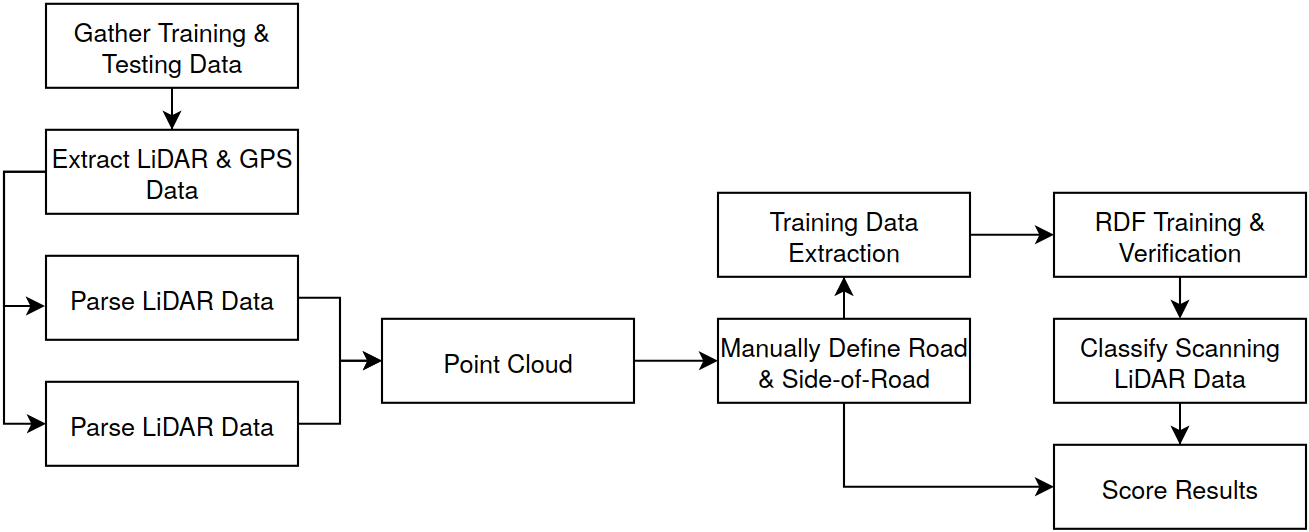
\includegraphics[width=0.9\linewidth]{figures/flowz_2}
				\caption[Project Flow]{High level view of project work}
				\label{fig:flowz_2}
			\end{figure}	
	
	%	\begin{figure}
		%		\centering
		%		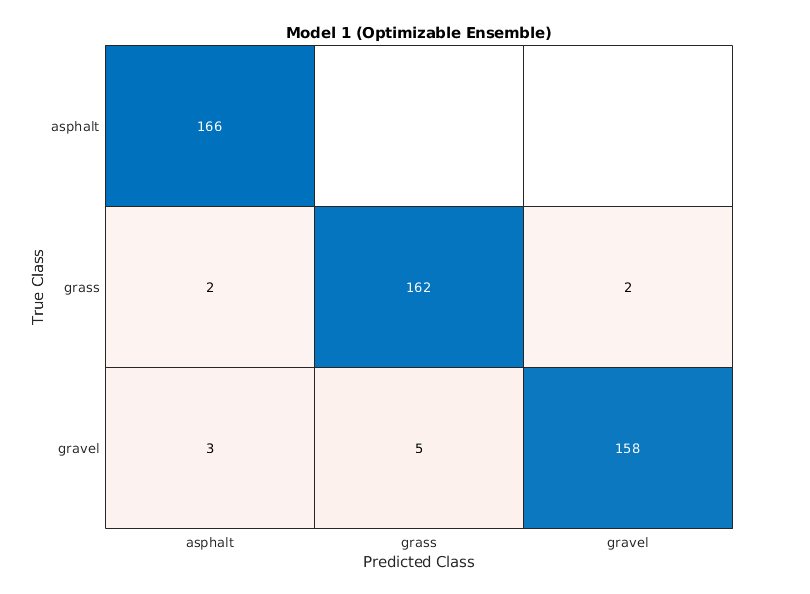
\includegraphics[width=\linewidth]{figures/test_conf_mat}
		%		\caption[Validation Confusion Matrix]{Confusion matrix from validation process.}
		%		\label{fig:vali_conf_mat}
		%	\end{figure}
	
		\subsection{Data Collection}
	
%	{The experimental apparatus for this work was the Ohio University Autonomous Van van (Fig. \ref{fig:Experimental_Apperatus}), which has a Velodyne VLP-32C scanning LiDAR sensor, Novatel PwrPak 7D-E2 GNSS and INS system, and Mako cameras. Raw data was gathered using the Robotic Operating System (ROS) to package incoming scanning LiDAR, GNSS, IMU, and camera sensor data as rosbags. Rosbags were unpacked using MATLAB tools to separate data streams. Prior to creating a training database, manual dictation of gravel and asphalt areas of the gathered point cloud data is necessary. In order to do so, all scanning LiDAR data from a rosbag was aggregated in order to create a single point cloud map. Scanning LiDAR timestamps were matched to the closest GNSS and IMU timestamp data. Closest matching GNSS and IMU data informed the location and orientation of the LiDAR scan (Fig. \ref{fig:road_areas_annotated_22}). Compiled point cloud maps was examined and compared to camera and satellite data to determine gravel and asphalt surface location. Manually defined 2D areas representing gravel and asphalt were projected unto the point cloud (Fig. \ref{fig:road_areas_annotated_22}).}
	
			{Required physical data was gathered by the Ohio University Autonomous Van (Fig. \ref{fig:Experimental_Apperatus}). LiDAR point cloud data was gathered with the vehicle's roof-mounted Velodyne VLP-32C. Velodnyne's VLP-32C has 32 channels producing 300,000 points per second with a vertical field of view from -45$^{\circ}$ to $+$15$^{\circ}$, providing a minimum 0.33$^{\circ}$ vertical angular resolution and 0.2$^{\circ}$ horizontal angular resolution \cite{vlp_32c}. GPS data was recorded with a Novatel PwrPak 7D-E2, a Global Navigation Satellite System (GNSS) \& Inertial Navigation System (INS), and two GNSS-502 antennas by NavtechGPS. Data acquisition and recording was completed on the vehicle's integrated Ubuntu 18.04 system using the Robot Operating System (ROS). Scanning LiDAR data of a gravel surface was gathered from a gravel parking lot (Fig. \ref{fig:gravel_training_lot}) near Athens Ohio. Scanning LiDAR data of an asphalt surface was gathered from Blackburn Road (Fig. \ref{fig:Blackburn_Road_View}) near the intersecting gravel lot. Scanning LiDAR data of grassy surfaces was gathered from the side of the gravel lot. Although this work does not evaluate the detection accuracy of grass, differentiation between a road and non-road surface is necessary for evaluating road-surface detection; therefore, grass is labeled as \textit{unknown} in this work. Raw data was gathered using the Robotic Operating System (ROS) to package incoming scanning LiDAR, GNSS, IMU, and camera sensor data as rosbags. Rosbags were unpacked using MATLAB tools to separate data streams. Point cloud, GPS, and IMU topics were defined, and point cloud Cartesian coordinates with corresponding intensities, longitude, latitude, altitude, roll, pitch, and yaw messages were read from the appropriate topics and imported.}
	
			\begin{figure}[H]
				\centering
				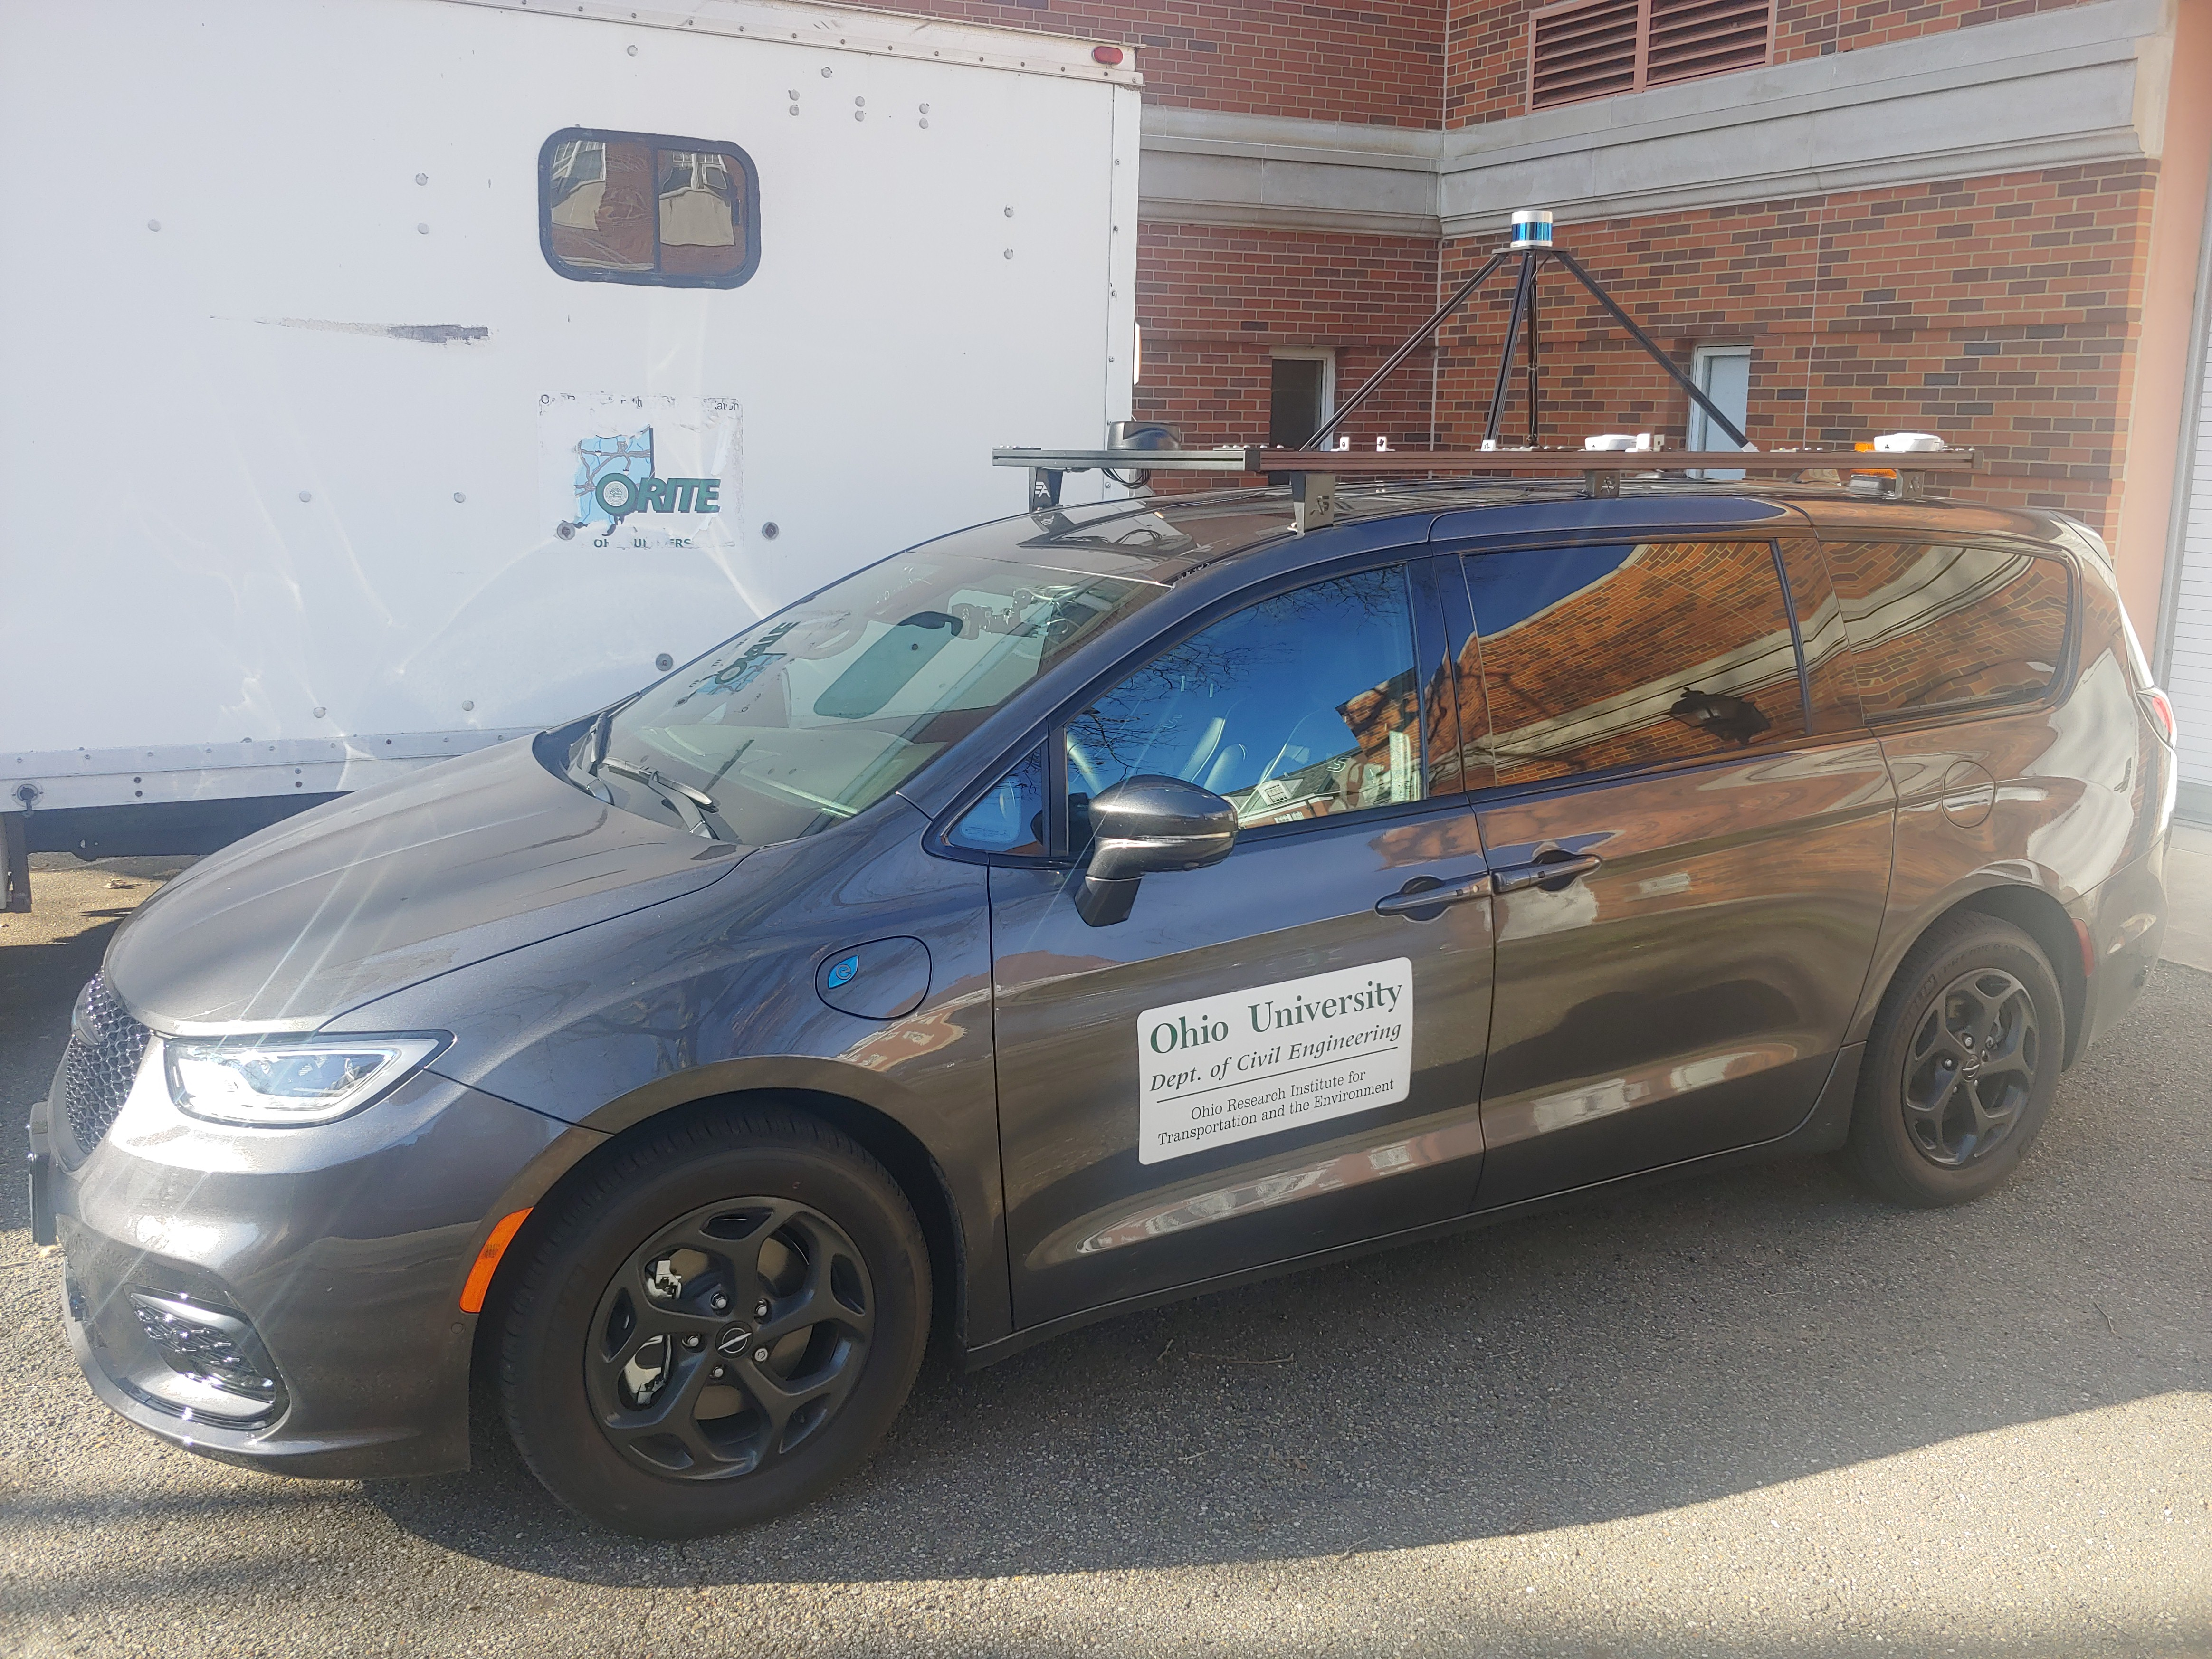
\includegraphics[width=0.75\linewidth]{figures/van_on_van}
				\caption[Experimental Apparatus]{Experimental Apparatus. Velodyne VLP-32 Scanning LiDAR is mounted on top of the vehicle.}
				\label{fig:Experimental_Apperatus}
			\end{figure}
		
			\begin{figure}[H]
				\centering
				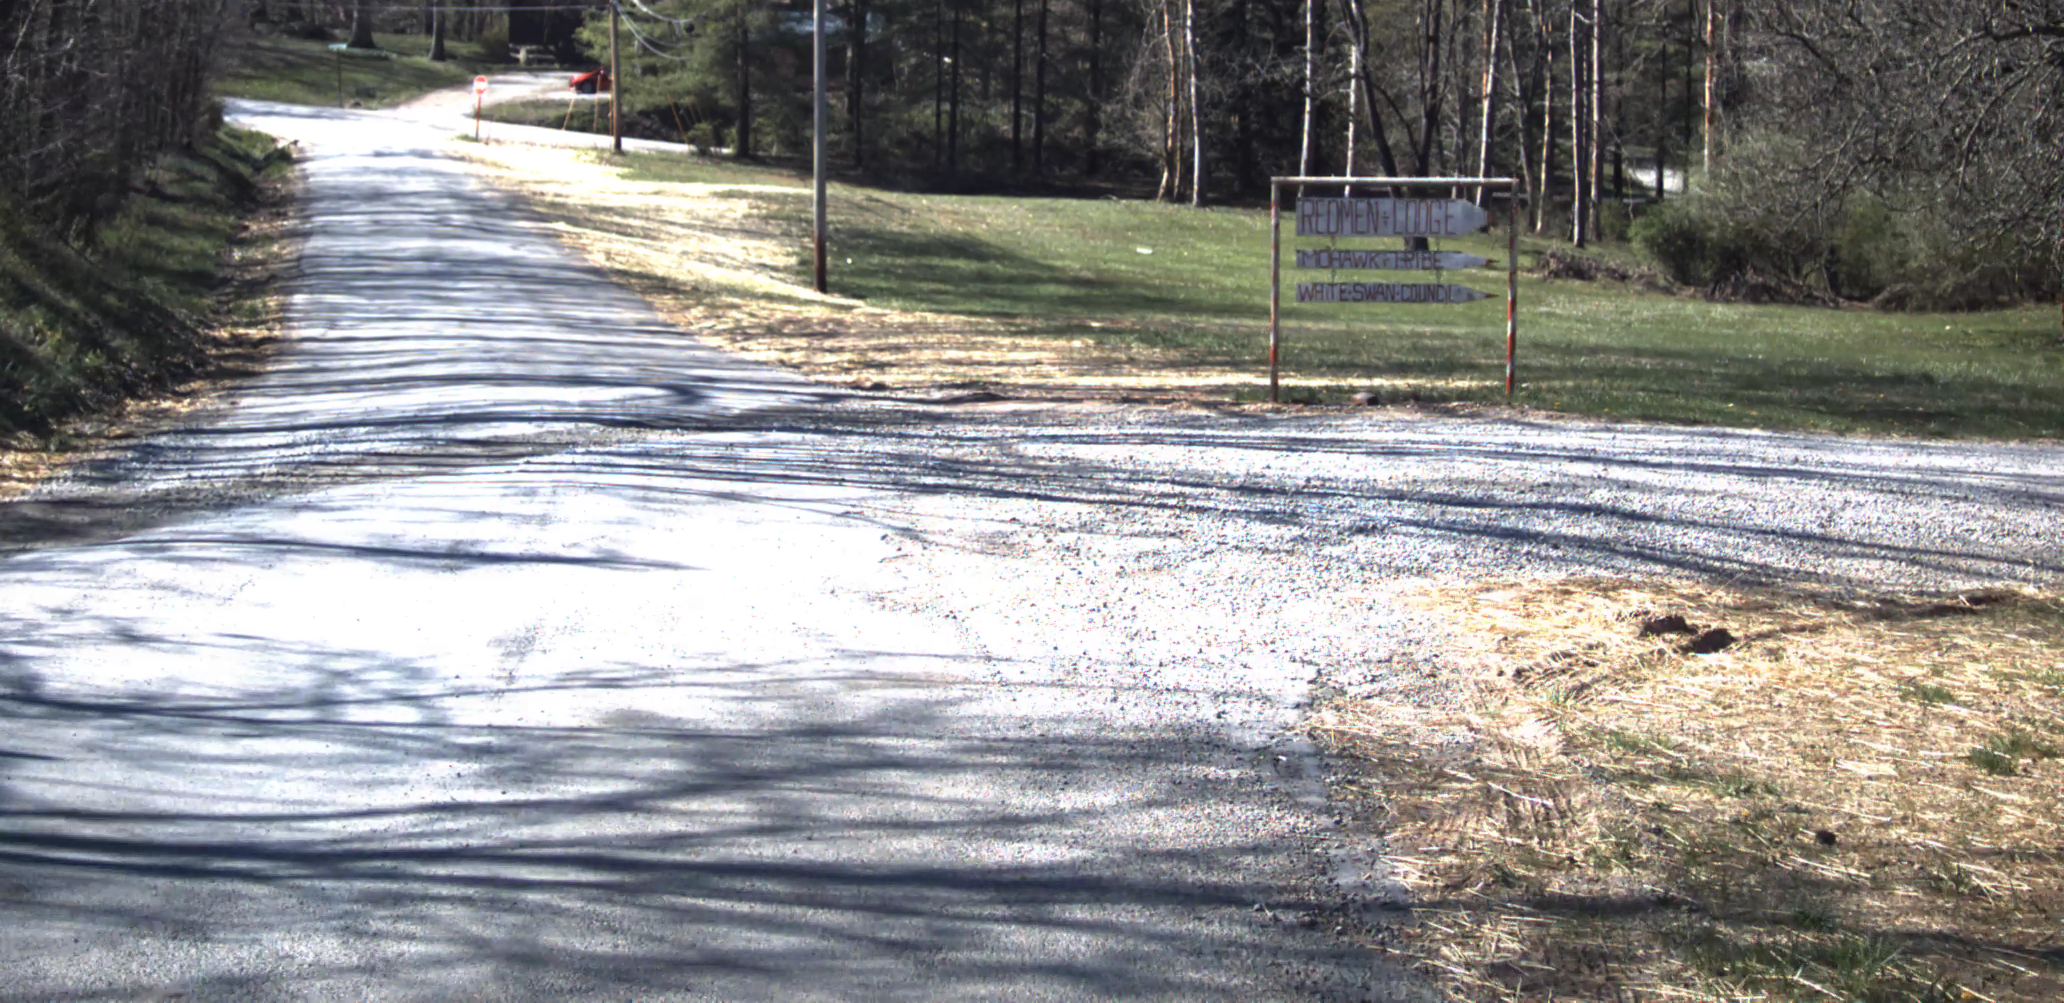
\includegraphics[width=0.75\linewidth]{figures/blackburn_road}
				\caption[Blackburn Road Camera View]{Camera view of Blackburn Road - an unmarked asphalt road with three intercepting gravel driveways from which asphalt data was gathered.}
				\label{fig:Blackburn_Road_View}
			\end{figure}
		
			\begin{figure}[H]
				\centering
				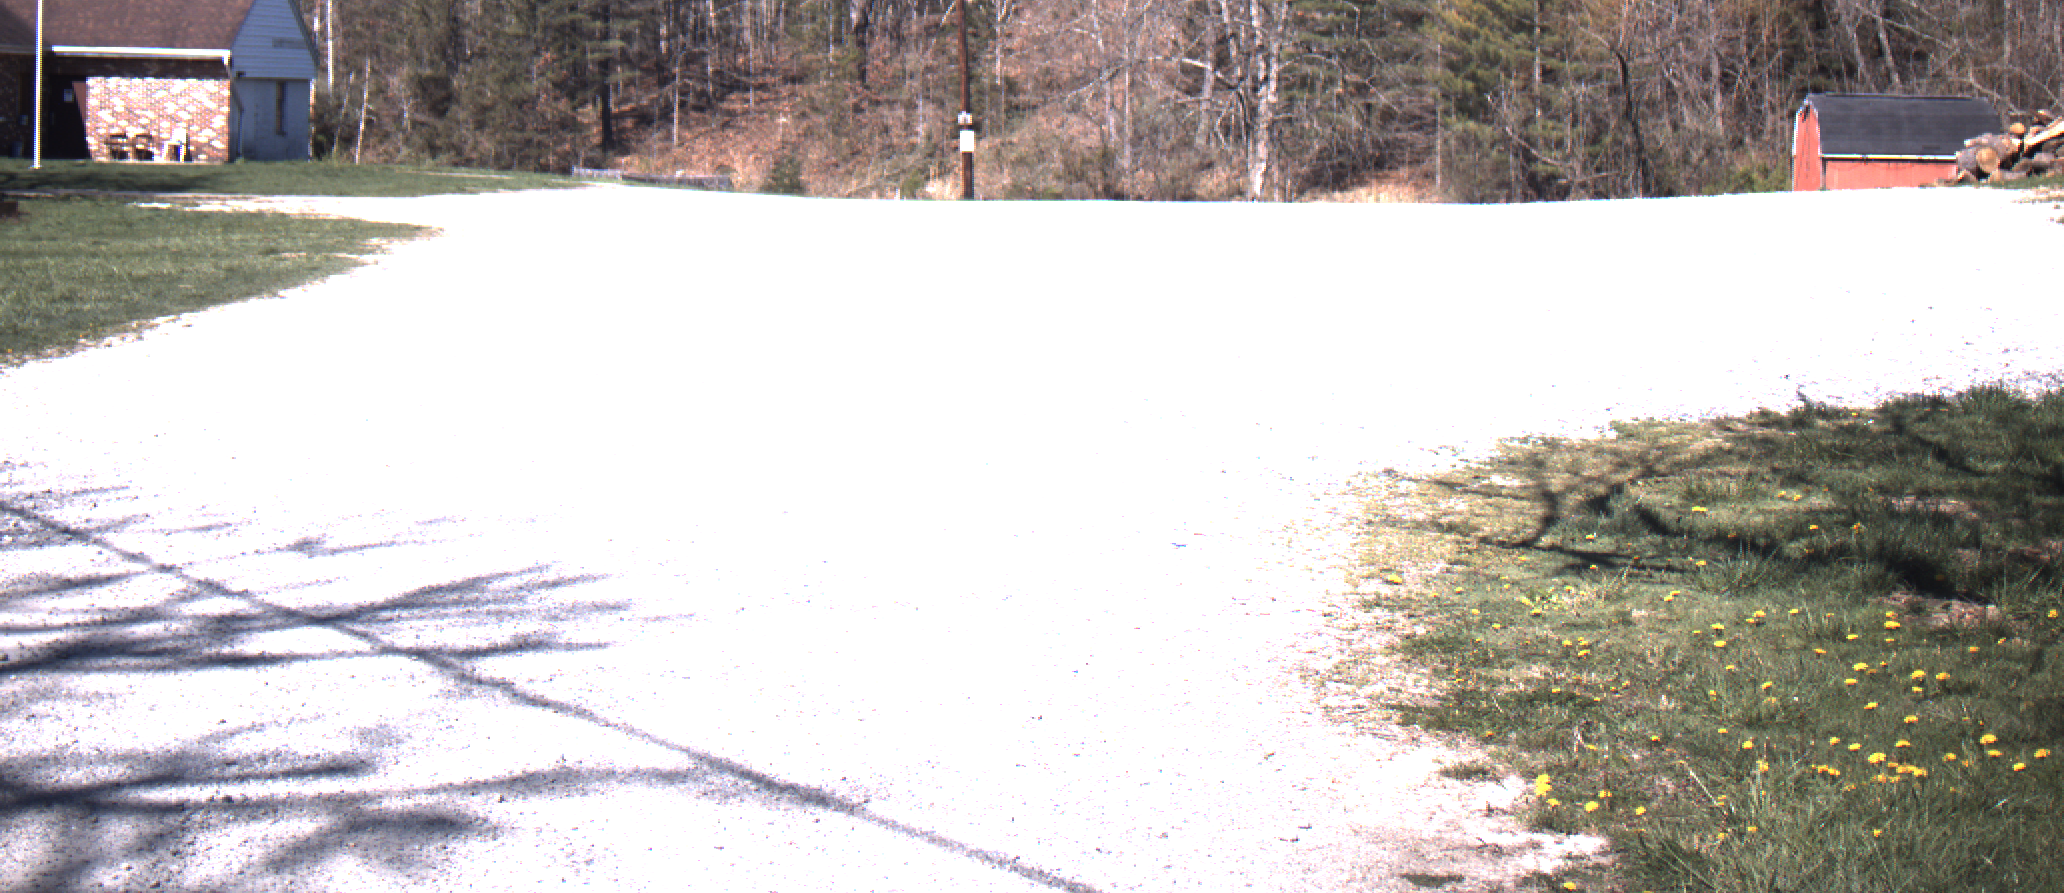
\includegraphics[width=0.75\linewidth]{figures/gravel_lot_pic}
				\caption[Gravel Training Lot]{Camera view of the gravel lot from which gravel training data was gathered.}
				\label{fig:gravel_training_lot}
			\end{figure}			
	

		\subsection{Training Data Extraction}
	
			{Scanning LiDAR training data requires extraction from manually defined \textit{gravel}, \textit{asphalt}, and \textit{unknown} terrain areas on aggregated point clouds. Aggregating LiDAR data into a single point cloud was completed by post processing rosbags that contained scanning LiDAR, GPS, and IMU data of an unmarked road. Scanning LiDAR timestamps were matched to the closest GNSS and IMU timestamp data. Closest matching GNSS and IMU data informed the location and orientation of the LiDAR scan. Point cloud translation and rotation was accomplished using transformation matrices derived from GPS and IMU data. Rotation matrices were created using extracted roll, pitch, and yaw data from the IMU. LiDAR origin was found using GPS longitude, latitude, and altitude data. Physical distances between the GPS, IMU, and LiDAR sensors were rectified by obtaining reference frames provided by AutonomouStuff. GPS coordinates were offset by the current orientation and converted the ground truth to the LiDAR frame. GPS, IMU, and LiDAR reference frames and rotational updates were combined into trajectory vectors. Consecutive point cloud scans were then translated and rotated with derived transformation matrices (Fig. \ref{fig:pc_example}). While not as robust as more sophisticated methods of point cloud aggregation, such as NDT or ICP scan matching, using this method proved to be adequate over shorter distances.}
			

			
			\begin{figure}[H]
				\centering
				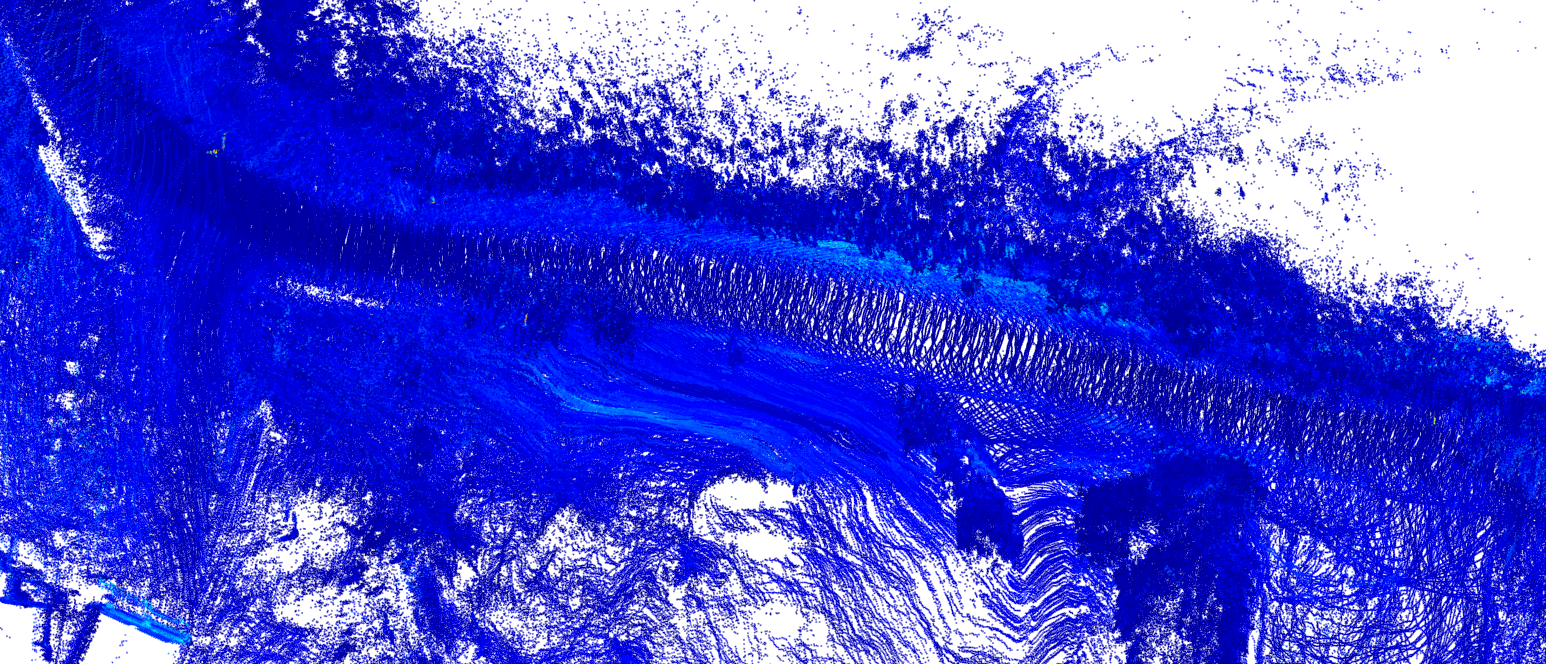
\includegraphics[width=0.75\linewidth]{figures/pc_example}
				\caption[Aggregated Point Cloud Data]{Point cloud of scanning LiDAR data using GPS and IMU data to determine point of origin and orientation for the LiDAR was used to create a combined point cloud map.}
				\label{fig:pc_example}
			\end{figure}
		
			{Manually defined areas were then overlayed onto the point cloud, representing training areas (Fig. \ref{fig:test_vs_train_areas}). Six degree arcs (Fig. \ref{fig:area_example}) from the first three channels of scanning LiDAR data directly in front of the vehicle were extracted and exported to a database if coincident with the manually defined areas. Training data was extracted from a single arc from each 360 degree LiDAR scan if the arc was coincident to a manually projected 2D area. Raw spatial and intensity values from the coincident arc were saved to a raw training database. Separate training databases were maintained for each individual channel. Features that describe the raw spatial and intensity data were extracted. Thirty percent of the training data base was randomly selected and set aside as a validation data base. Training data was visually examined for clustering to verify that a RDF would be able to be trained (Fig. \ref{fig:training_data_cluster_2}). It was found that each class generally clustered to a certain range with some overlap, which indicates that a RDF may be trained.}
			
			\begin{figure}[H]
				\centering
				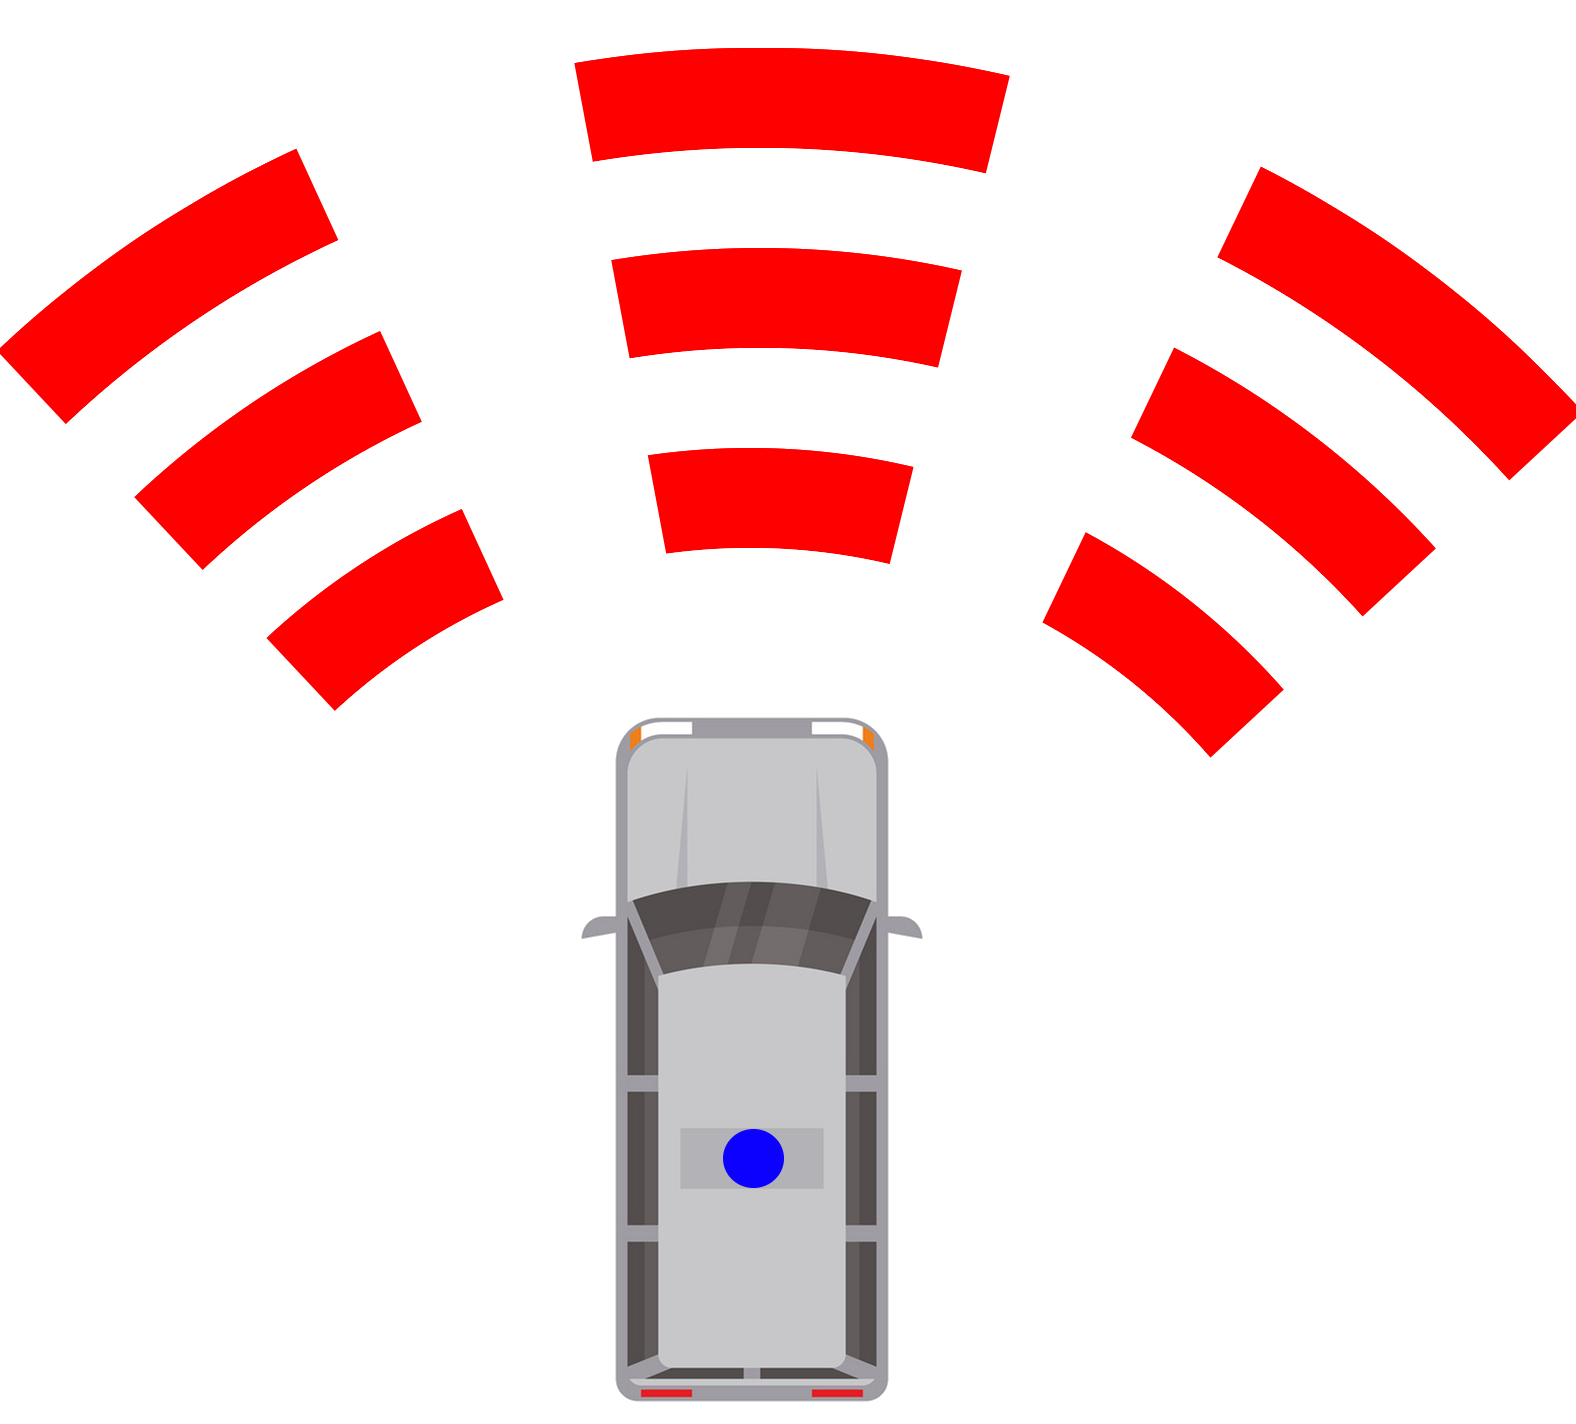
\includegraphics[width=0.25\linewidth]{figures/area_example}
				\caption[Areas to Classify]{Three arcs from three channels were classified per 360 degree scan. }
				\label{fig:area_example}
			\end{figure}
		
			\begin{figure}[H]
				\centering
				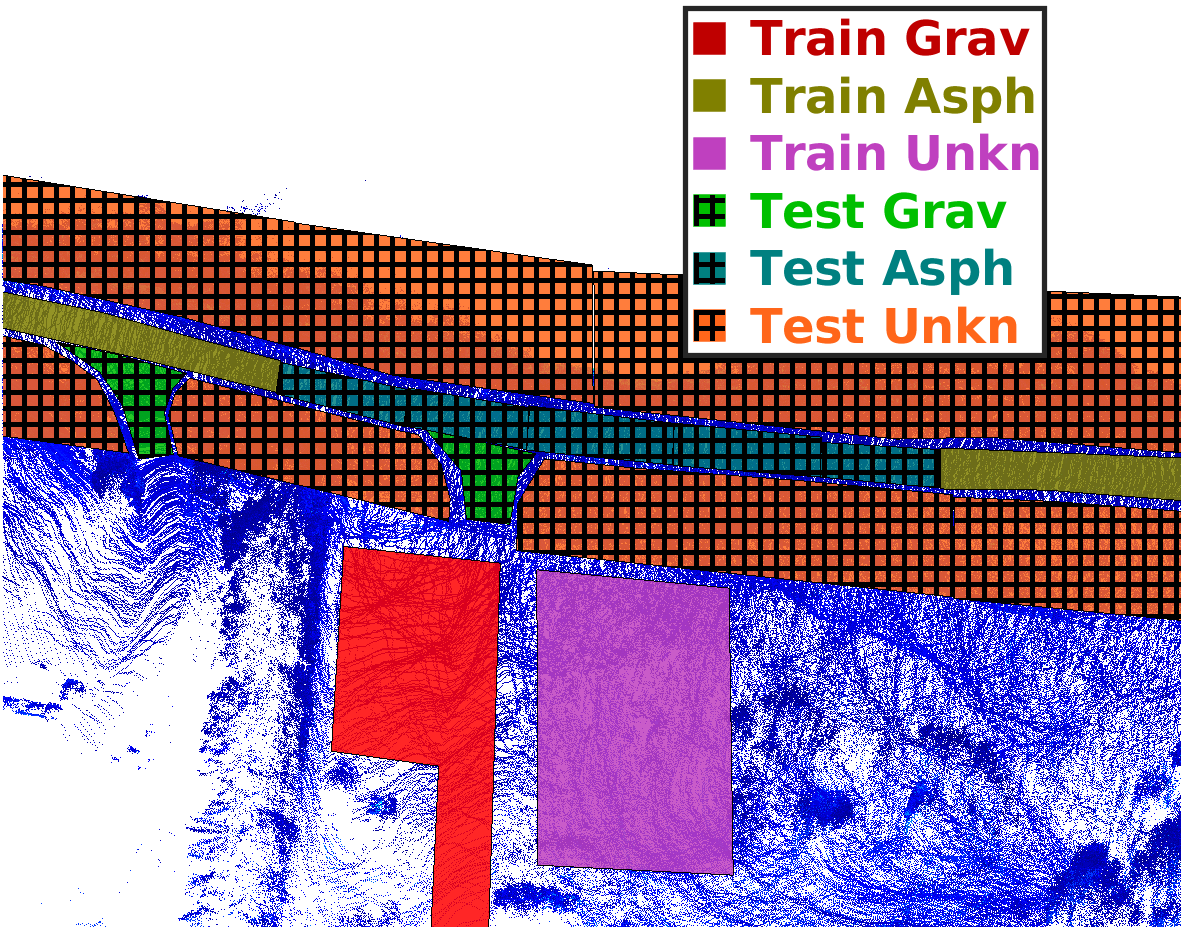
\includegraphics[width=0.75\linewidth]{figures/test_vs_train_areas_hatch}
				\caption[Training vs Testing Areas]{Training areas were kept separate from the testing areas.}
				\label{fig:test_vs_train_areas}
			\end{figure}
			
%			\begin{figure}[H]
%				\centering
%				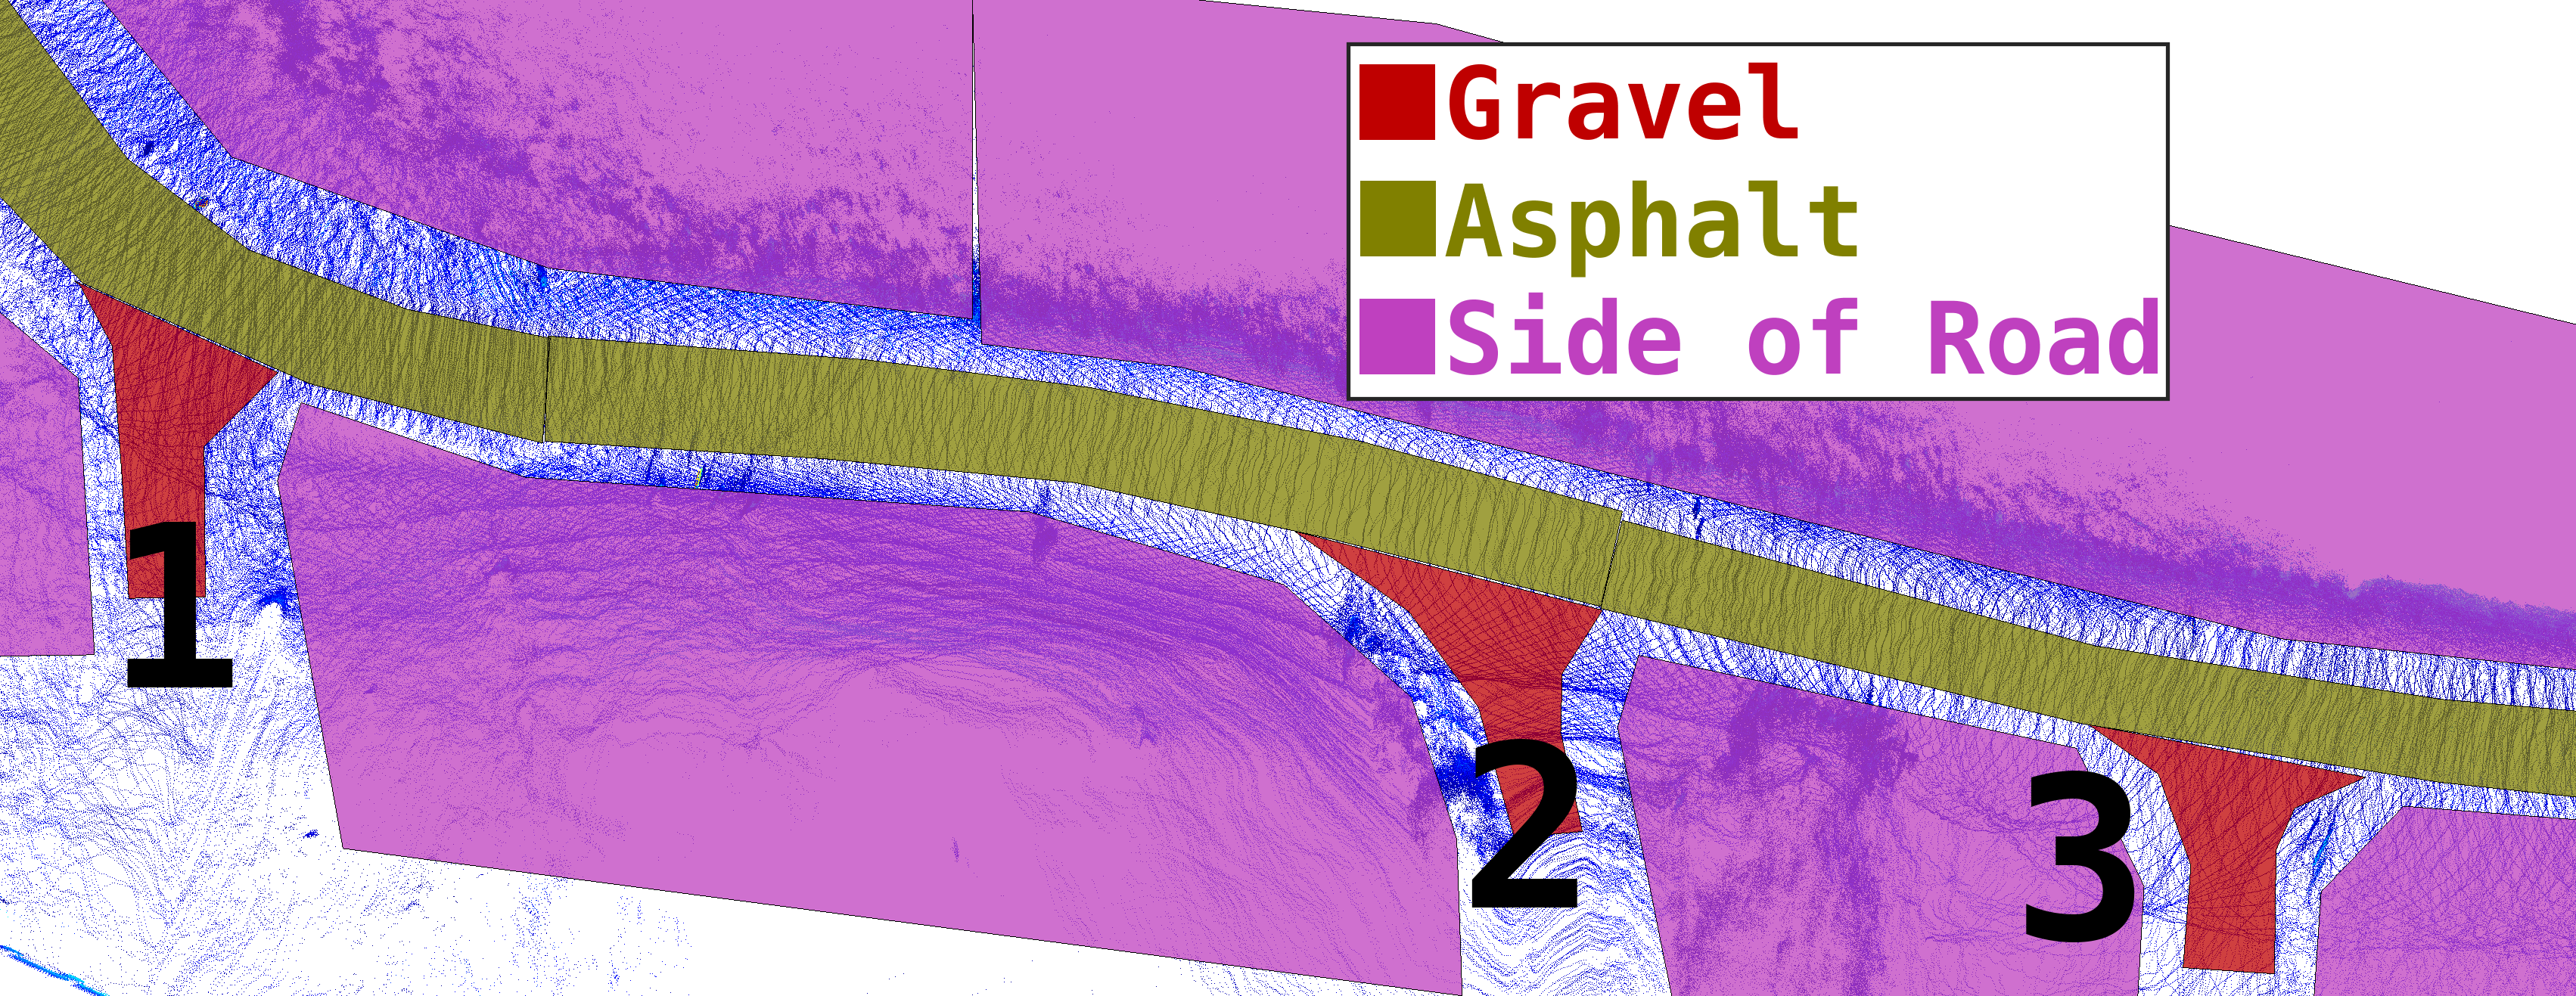
\includegraphics[width=0.75\linewidth]{figures/road_areas_annotated_2}
%				\caption[Manually Classified Point Cloud Data]{ Projected manually defined areas define terrain surface type. Three gravel driveways (annotated 1-3) intercept an asphalt road, area $3$ is the gravel parking lot entrance from which training data was extracted.}
%				\label{fig:road_areas_annotated_22}
%			\end{figure}

			\begin{figure}[H]
			\centering
			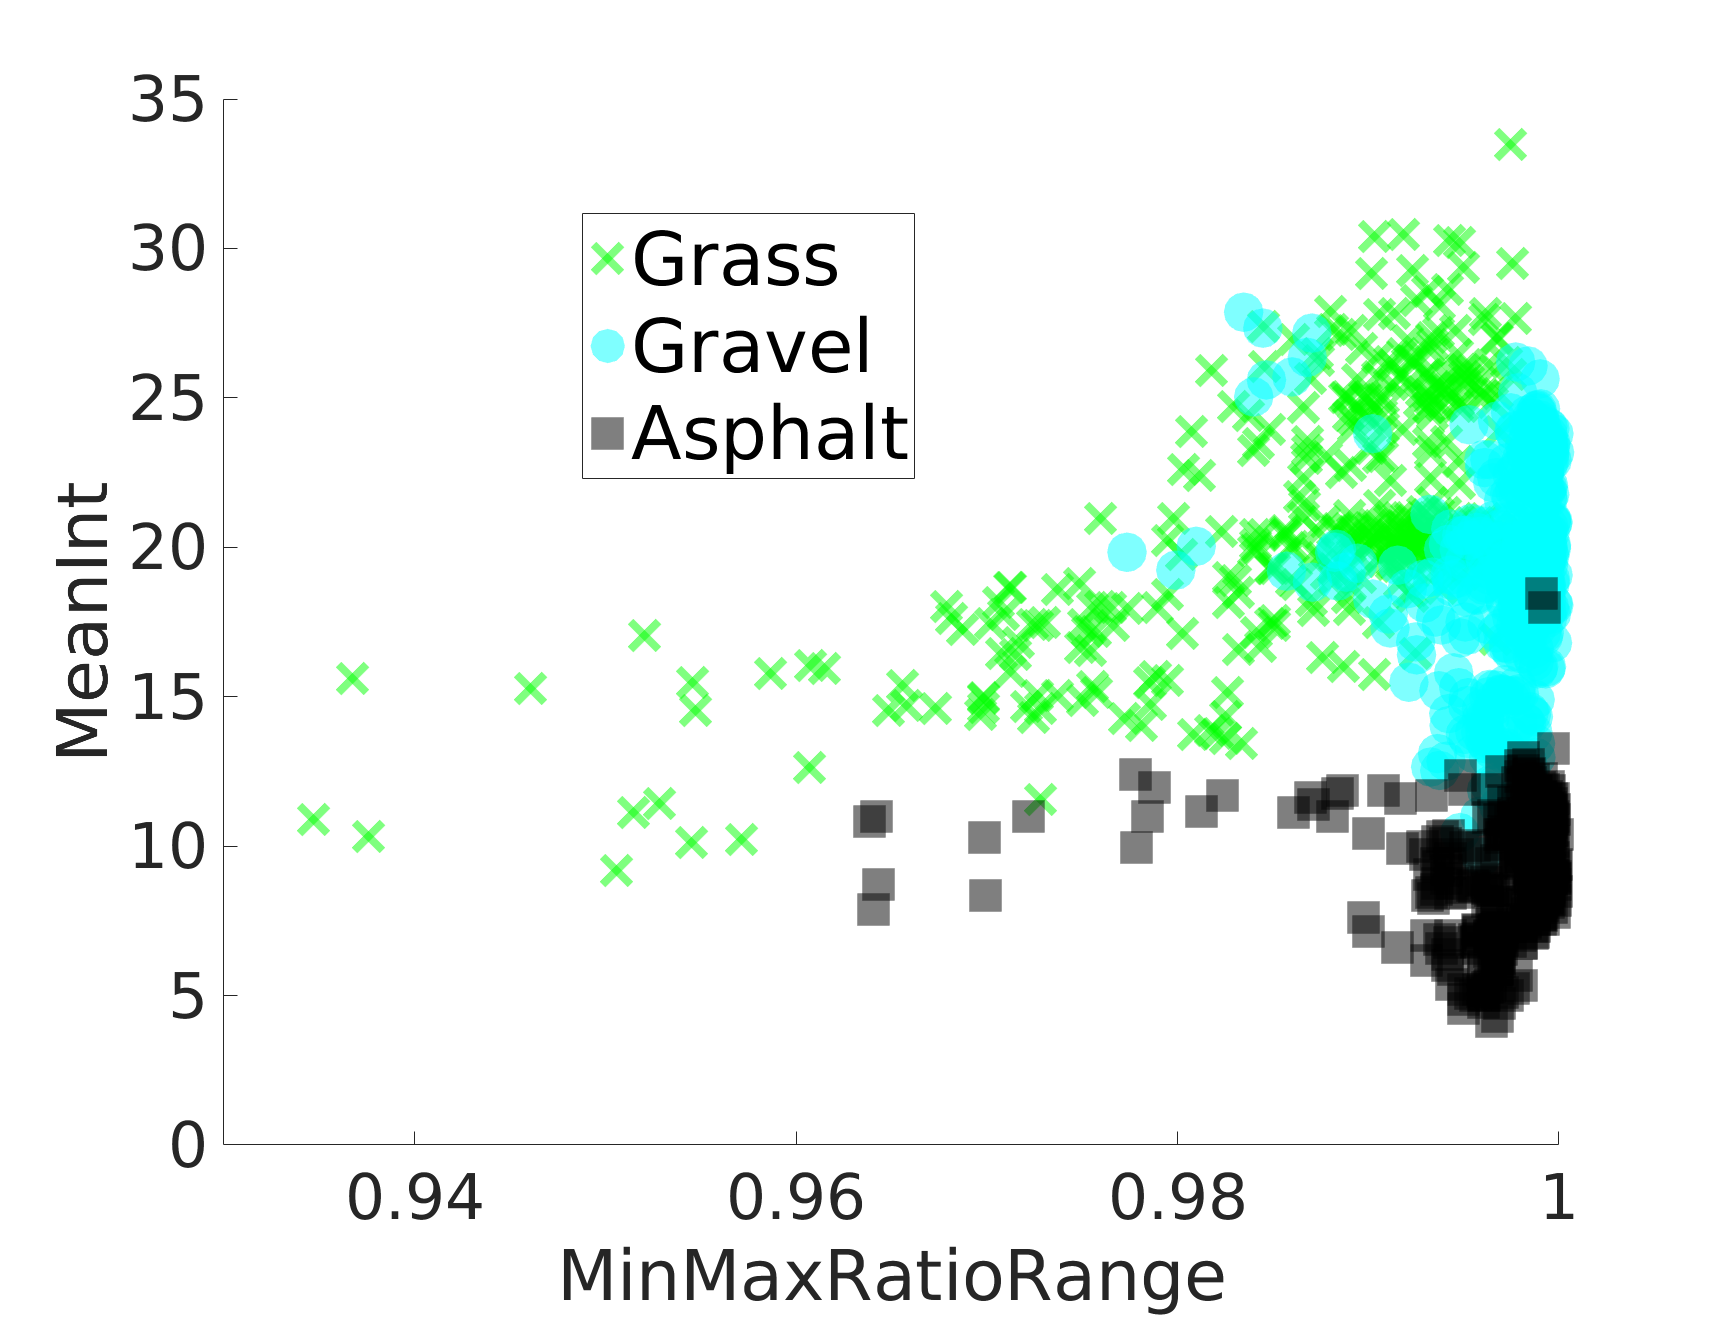
\includegraphics[width=0.75\linewidth]{figures/training_data_cluster_3}
			\caption[Example Clustering]{Example of training data comparison between two features.}
			\label{fig:training_data_cluster_2}
			\end{figure}
	
			{LiDAR returns spatial data represented by Cartesian coordinates with units in meters and remission data represented by a dimensionless ratio of minimum to maximum detected brightness. Feature extraction was completed by performing mathematical functions on the gathered spatial training data, yielding the Standard Deviation ($\sigma$), Roughness ($max - min$), Min-Max Ratio ($min / max$), Min$^{2}$-Max Ratio ($min^2 / max$), and Gradient ($sqrt(\sum_{1}^{n} G))$), where $G$ is an $1*n$ array comprising of the differences between consecutive points in the spatial data array. Spatial features were non-dimensionalized as necessary by dividing the average range of the arc to LiDAR point of origin to the appropriate power. Remission features include Standard Deviation ($\sigma$), Mean, Roughness ($max - min$), Min-Max Ratio ($min / max$), Min$^{2}$-Max Ratio ($min^2 / max$), and Gradient ($sqrt(\sum_{1}^{n} G))$). As remission is a ratio of minimum to maximum detectable reflected intensity, there was no need to render the features non-dimensionalized. Thirty percent of the training data was randomly selected and reserved to create a validation data set.} 
	
	% When the app performs hyperparameter tuning by using Bayesian optimization (see Optimization Options for a brief introduction), it chooses the set ofhyperparameter values that minimizes an upper confidence interval of the classification error objective model, rather than the set that minimizes the classification error.
	
		\subsection{RDF Training and Testing}
		
			%MATLAB was used to train a Random Decision Forests for each of the three considered channels using Bayesian Optimization to tune tree depth and number of splits. Training continued until a minimum error was reached (Fig. \ref{fig:c2_min_class_error}). Validation of the RDF was then completed using the validation database.
	
			{MATLAB's Classification Learner Application was used to generate an RDF for each considered scanning LiDAR channel. Decision tree depth, number of learners, and number of features to consider for each binary split are hyper-parameters that were optimized using MATLAB's Bayesian Optimization. Bayesian Optimization automates the manual hyper-parameter tuning process by creating a surrogate model representing the objective function, in this case the upper confidence interval of the classification error objective model (Fig. \ref{fig:c2_min_class_error}). Initialization of the objective function is completed by training a number of RDFs using randomly selected hyper-parameters. Out-of-bag error is then found and used to create a series of Gaussian curves. Additional hyper-parameter values are chosen by an acquisition function to determine their utility in minimizing out-of-bag error. After a set number of iterations, best hyper-parameters are chosen based on minimum upper confidence interval of the classification error objective model. Hyperparameter tuning may lead to over-fitting to the training data base. Testing for over-fitting was accomplished by comparing the out-of-bag training error to the validation error (Fig. \ref{fig:train_vs_valid_overfit_test2}). Confusion matrices provide validation database classification accuracy information by classifying each data set in the validation database and comparing actual and predicted classes, resulting in a matrix that visualizes the accuracy for each terrain type as well as which terrain types are more likely to be confused for a different class (Fig. \ref{fig:vali_err_conf_mat}). This process was completed for each of the three considered scanning LiDAR channels used for classification.}
	
			\begin{figure}[H]
				\centering
				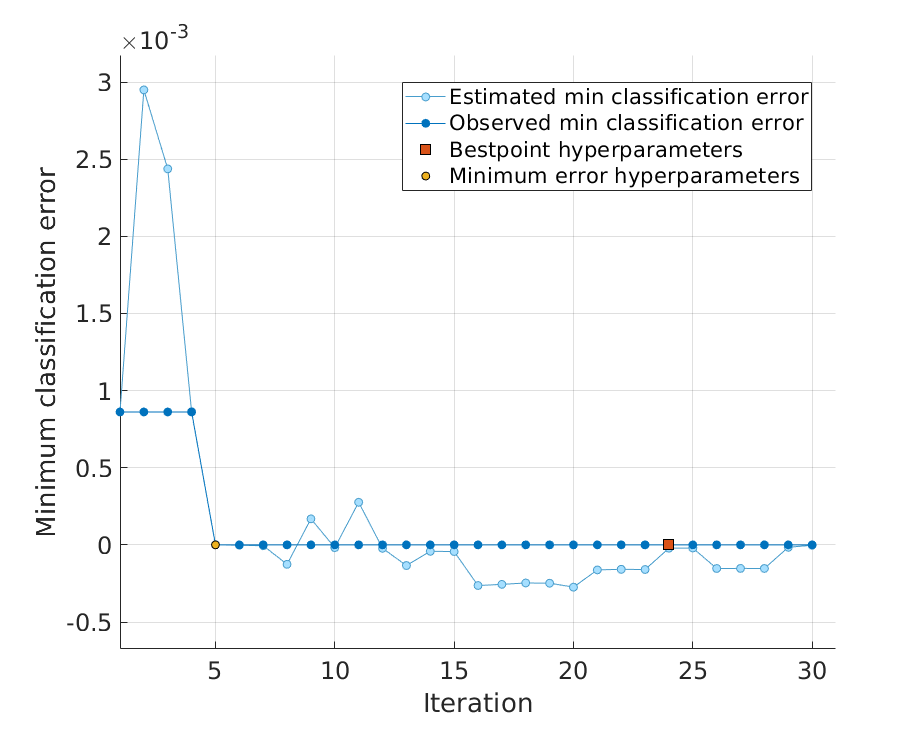
\includegraphics[width=0.75\linewidth]{figures/c2_min_class_error}
				\caption[RDF Training Classification Error]{Classification error during Bayesian Optimization tuning. Best hyper-parameters are chosen based on minimum upper confidence interval of the classification error objective model, not minimum classification error.}
				\label{fig:c2_min_class_error}
			\end{figure}
		
			\begin{figure}[H]
				\centering
				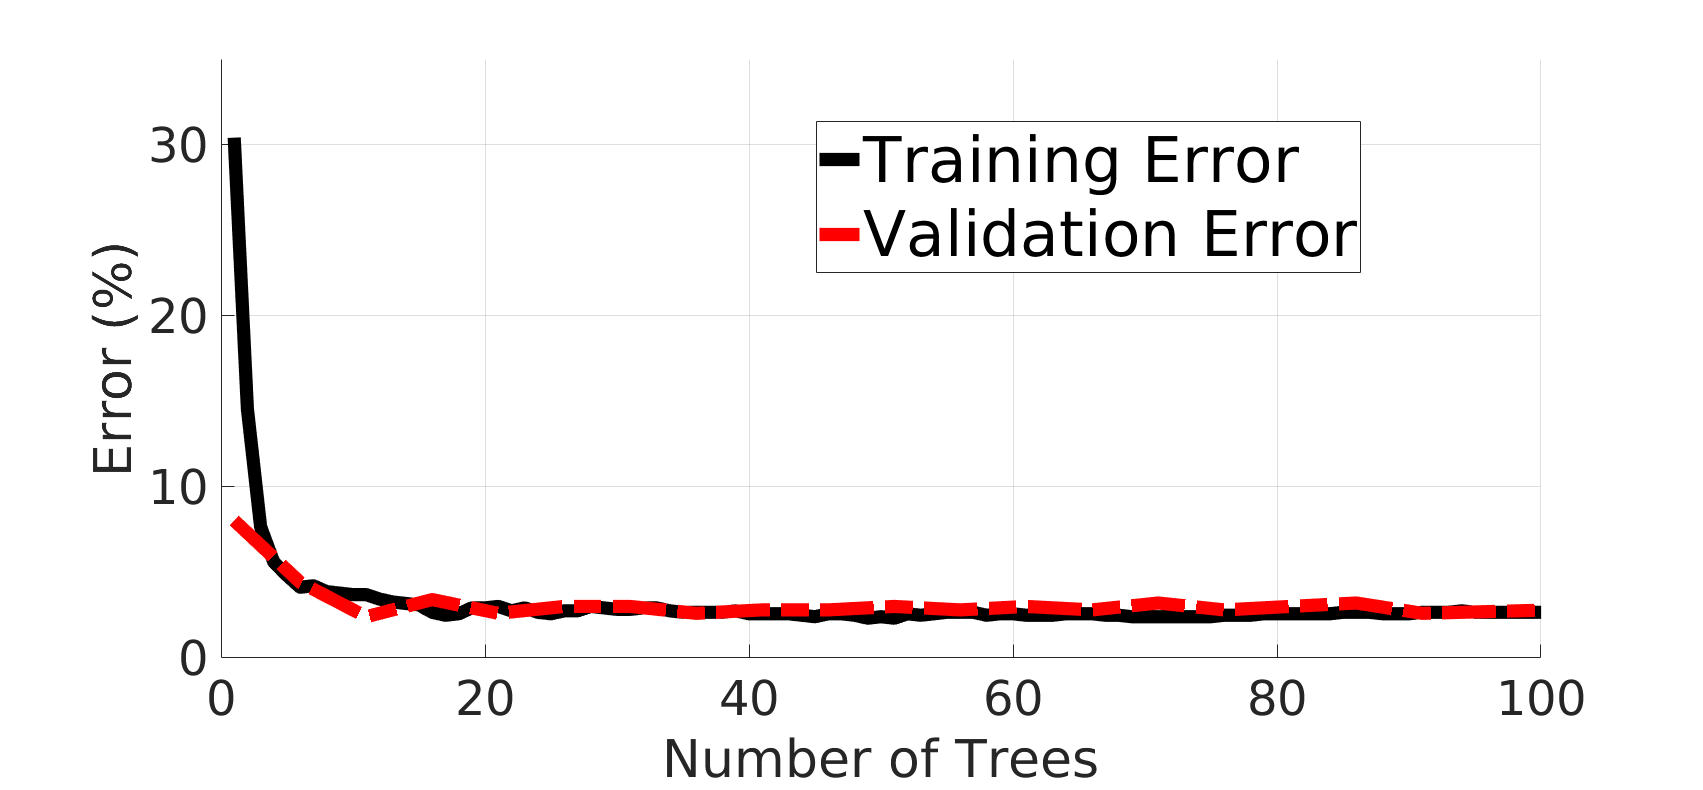
\includegraphics[width=0.75\linewidth]{figures/train_vs_valid_overfit_test3}
				\caption[Training vs Validation Error]{Hyper-parameter tuning may lead to over-fitting. Testing out-of-bag versus validation error demonstrates that the model is not over-fitting to the training data base if the validation error does not diverge from the out-of-bag error.}
				\label{fig:train_vs_valid_overfit_test2}
			\end{figure}
		
%			\begin{figure}[H]
%				\centering
%				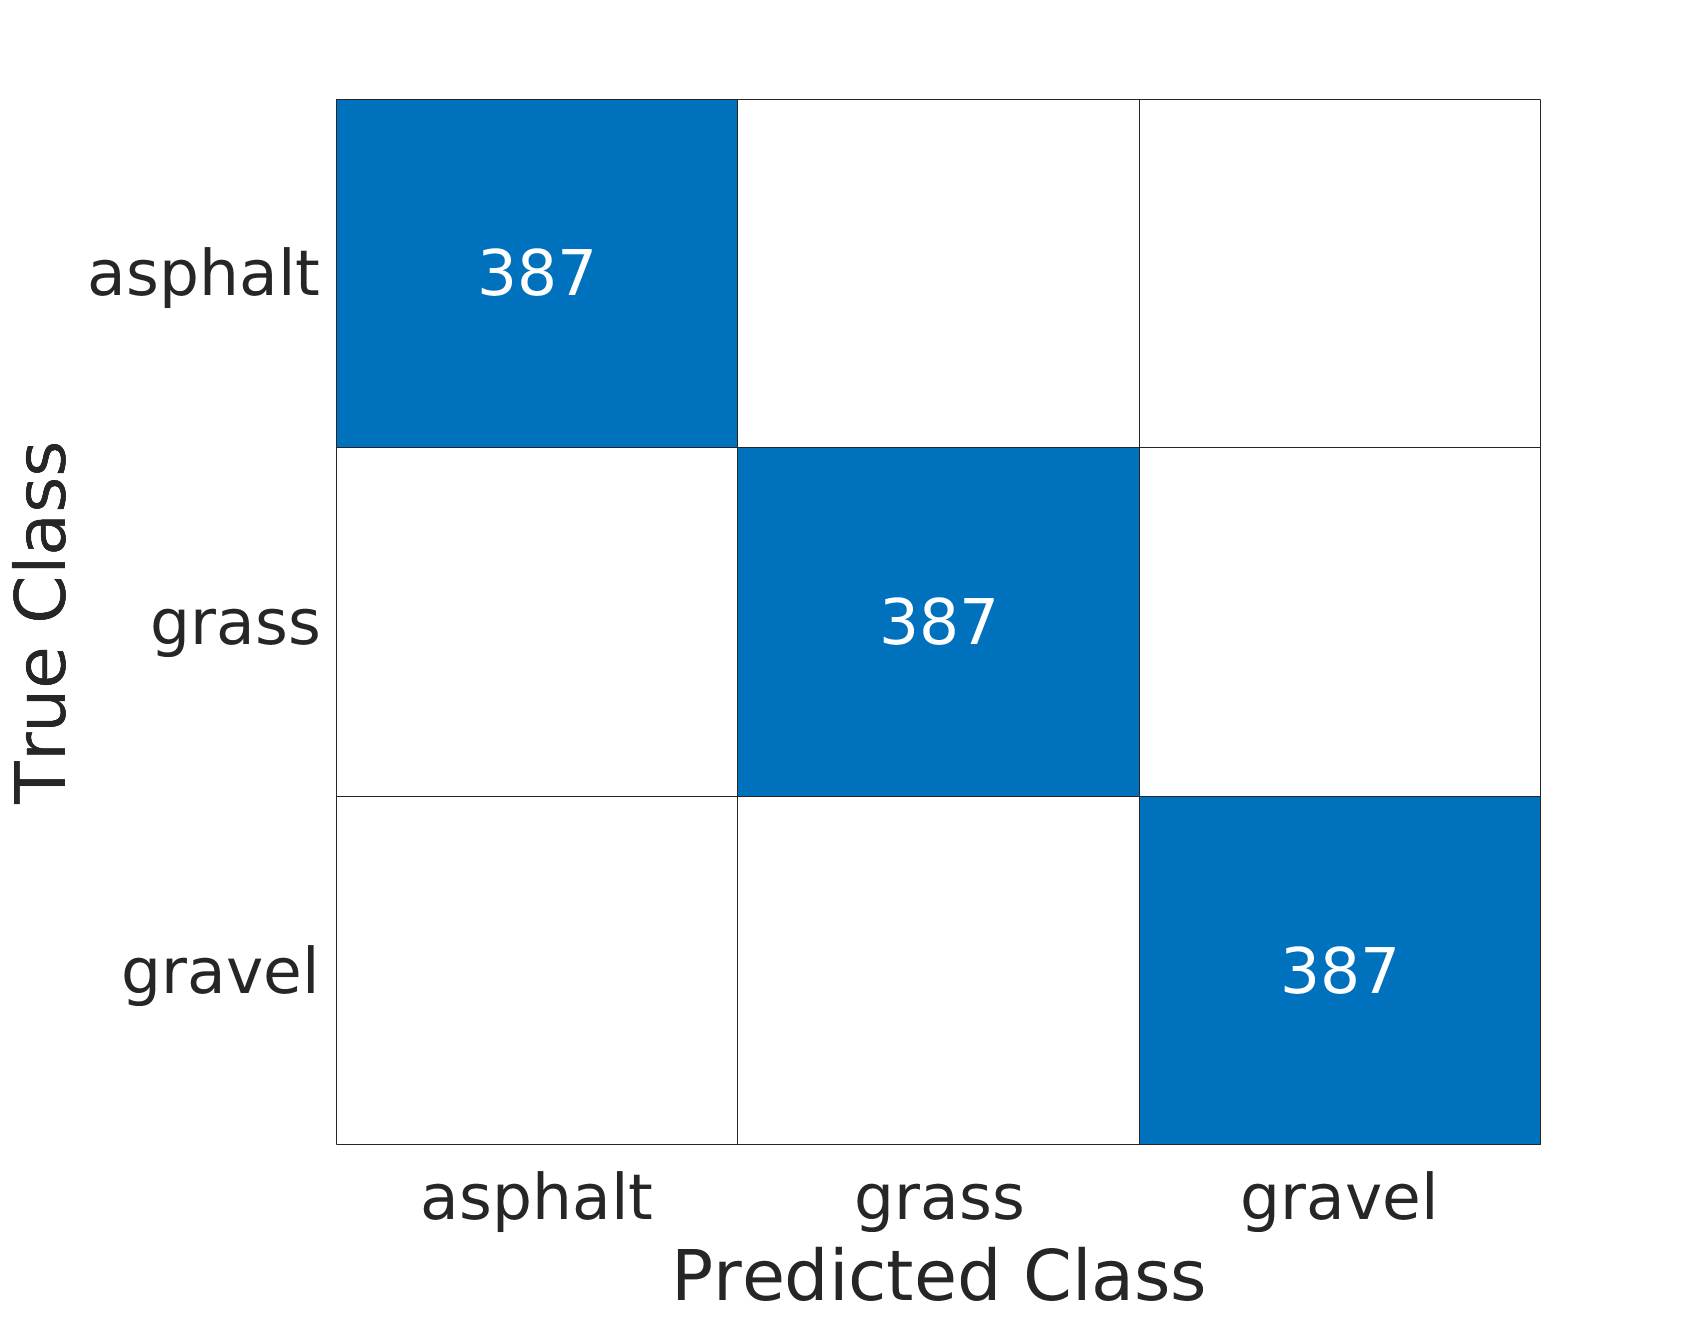
\includegraphics[width=0.75\linewidth]{figures/chan_2c_conf_OOB_mat222}
%				\caption[Out-of-Bag Error]{During training the RDF may be tested using the out-of-bag error. Confusion matrices are used to indicate the final RDF iteration training error.}
%				\label{fig:out_of_bag_err_conf_mat}
%			\end{figure}
		
			\begin{figure}[H]
				\centering
				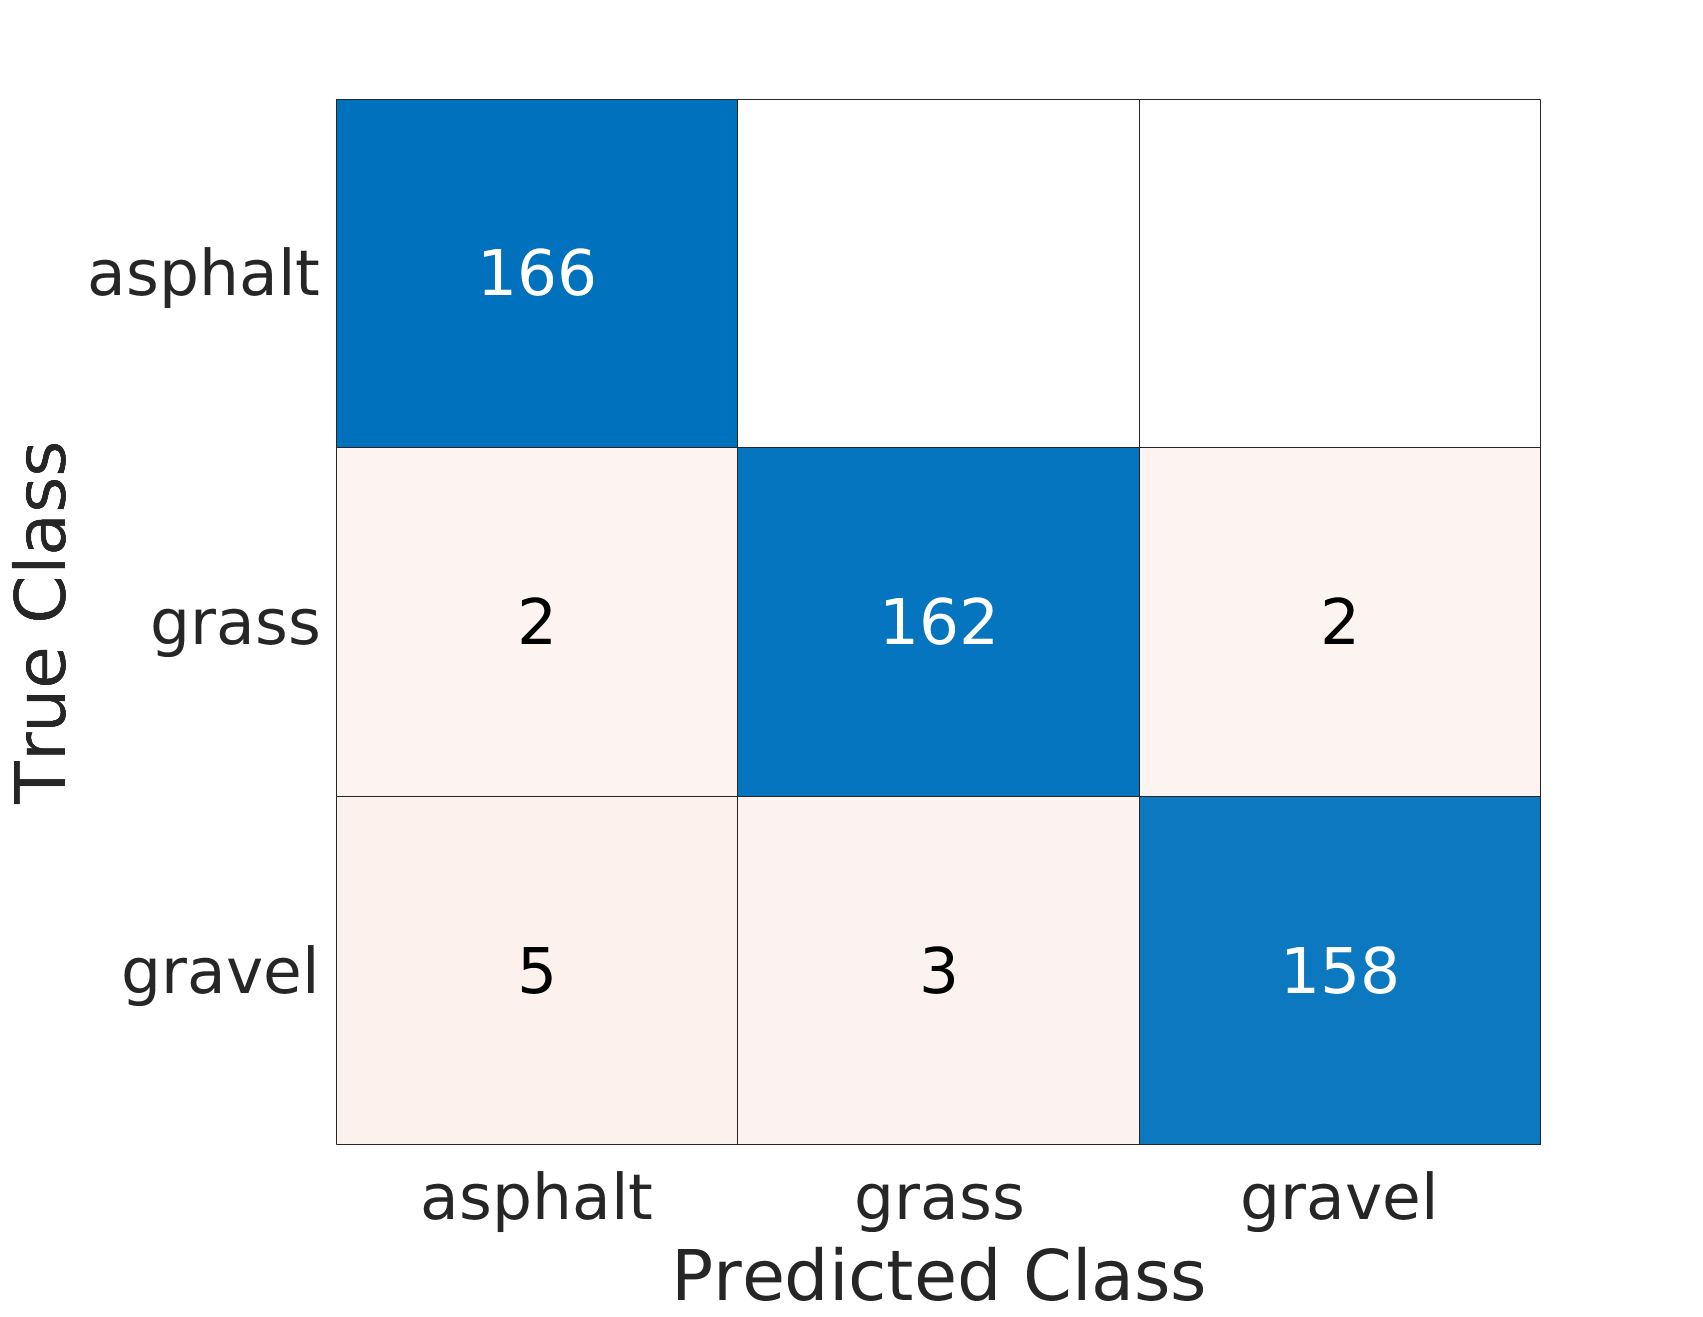
\includegraphics[width=0.55\linewidth]{figures/chan_2c_conf_VALIDATION_mat222}
				\caption[Validation Error]{Confusion matrix with the validation training data set.}
				\label{fig:vali_err_conf_mat}
			\end{figure}			
			
			{Classifying consecutive LiDAR scans was accomplished by examination of the nine arcs of interest in front and forty-five degree angles left and right from the front of the experimental apparatus (Fig. \ref{fig:area_example}). Features from each arc were extracted and the arc was classified (Fig. \ref{fig:raw_classification_results} shows the average spatial coordinates of each classified arc). Previously-created manually defined gravel, asphalt, and side-of-road truth areas (denoted as Testing areas in Fig. \ref{fig:test_vs_train_areas}) were projected onto the classified point cloud for the determination of classification accuracy. Averaged x, y, and z coordinates were taken of each arc, and projected unto a manually defined truth area map (Fig. \ref{fig:rm_db_4_toc}). Accuracy scores was calculated based on the distribution of classified points with each area, allowing evaluation of unmarked road detection performance. Classified point clouds were visually inspected to determine if the manual detection of a road surface may be accomplished. If consecutive points from each channel in any direction had two or more matching gravel or asphalt classification and was evenly spaced, a gravel or road surface area was projected. Guessed road surface areas were then compared to actual areas to determine the method's ability at unmarked gravel road discovery, indicating the method's efficiency at detecting intersecting gravel roads. }
			
			\begin{figure}[H]
				\centering
				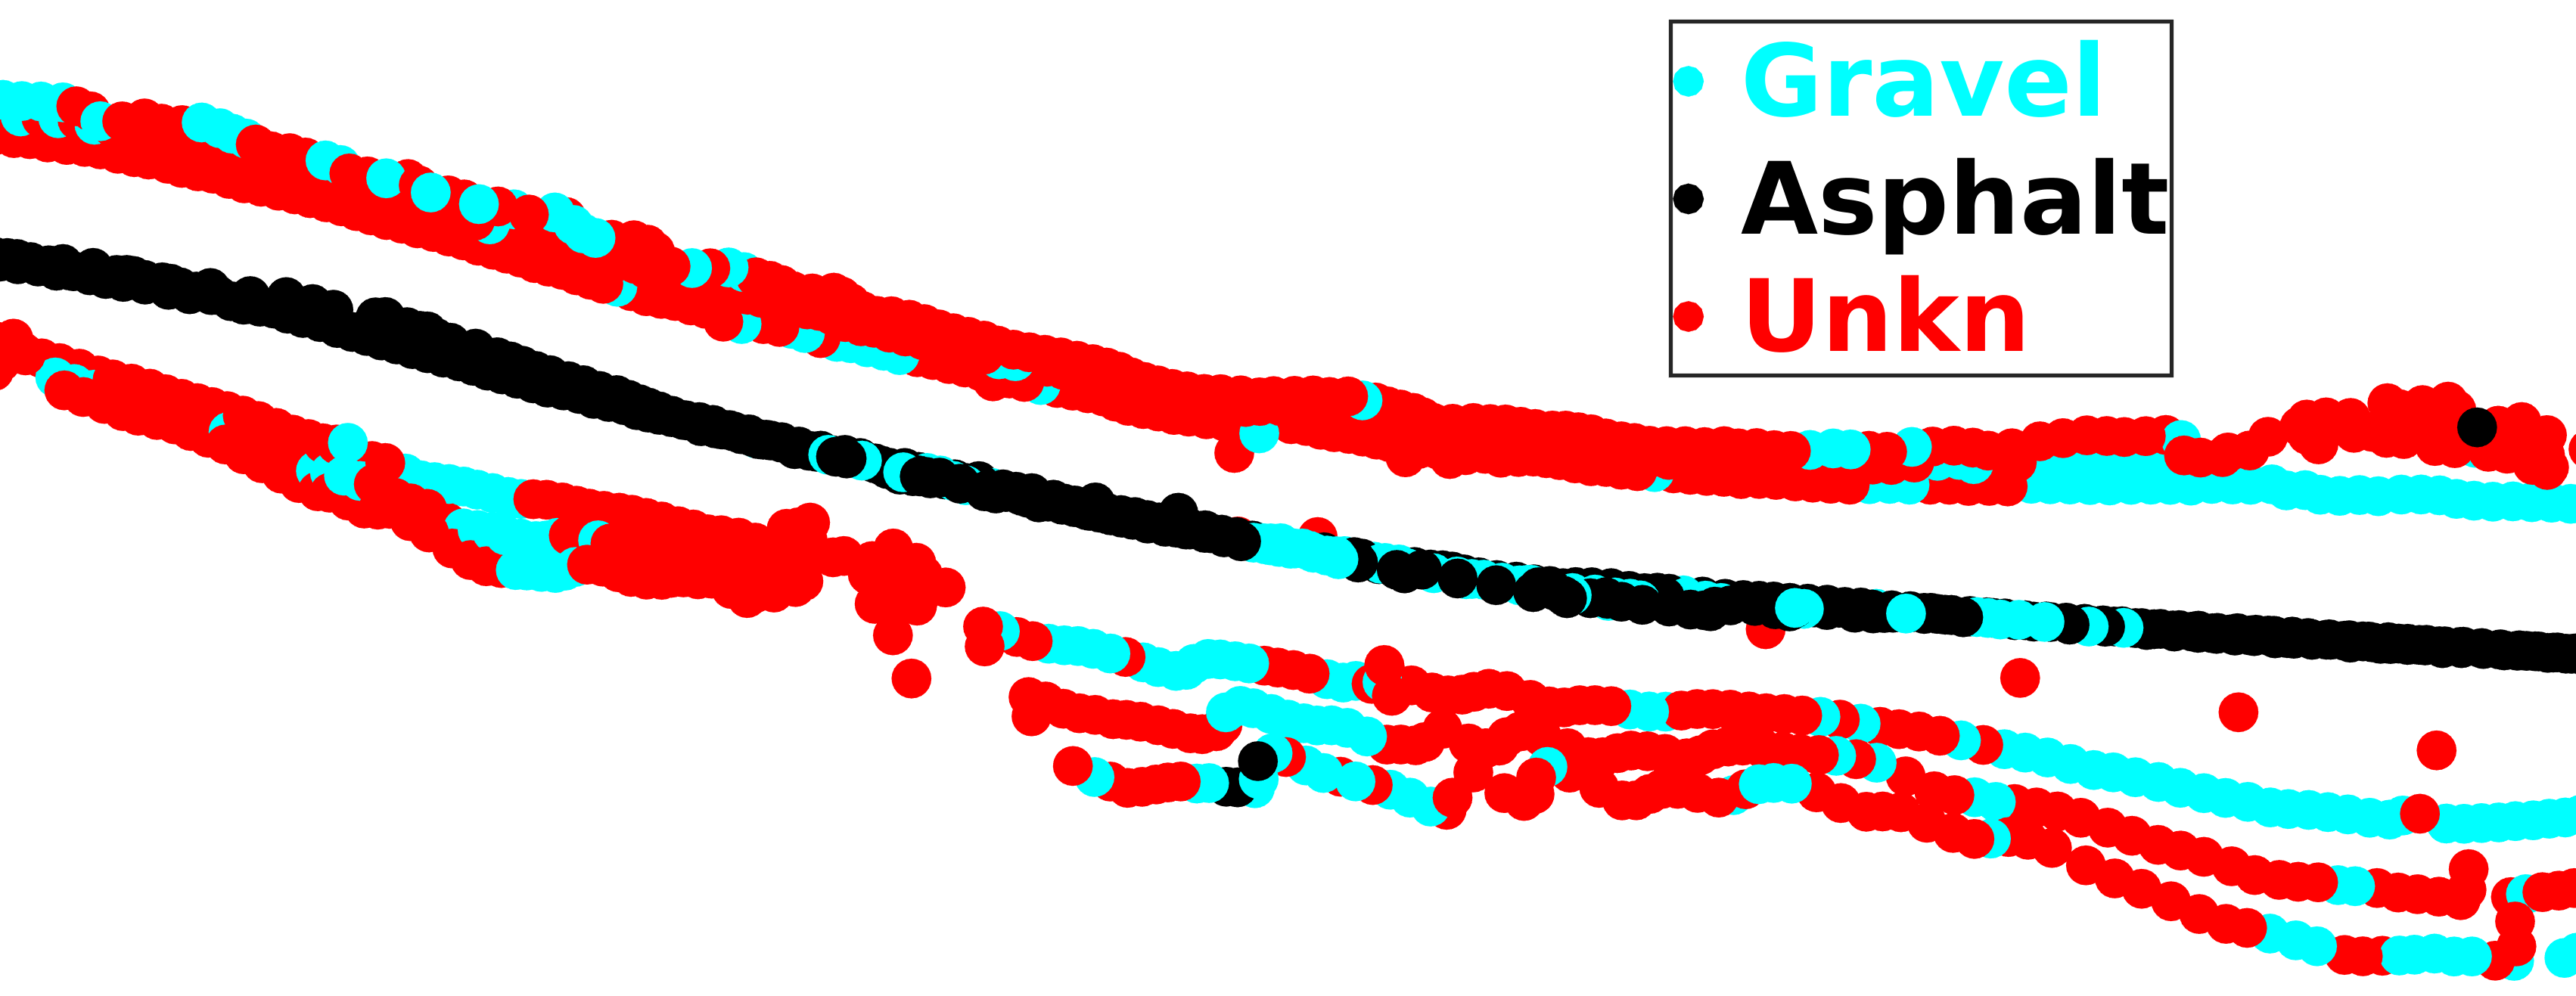
\includegraphics[width=0.9\linewidth]{figures/range_classified_pc_db_6}
				\caption[Classified Point Cloud]{Classified Point Cloud.}
				\label{fig:raw_classification_results}
			\end{figure}
		
			\begin{figure}[H]
				\centering
				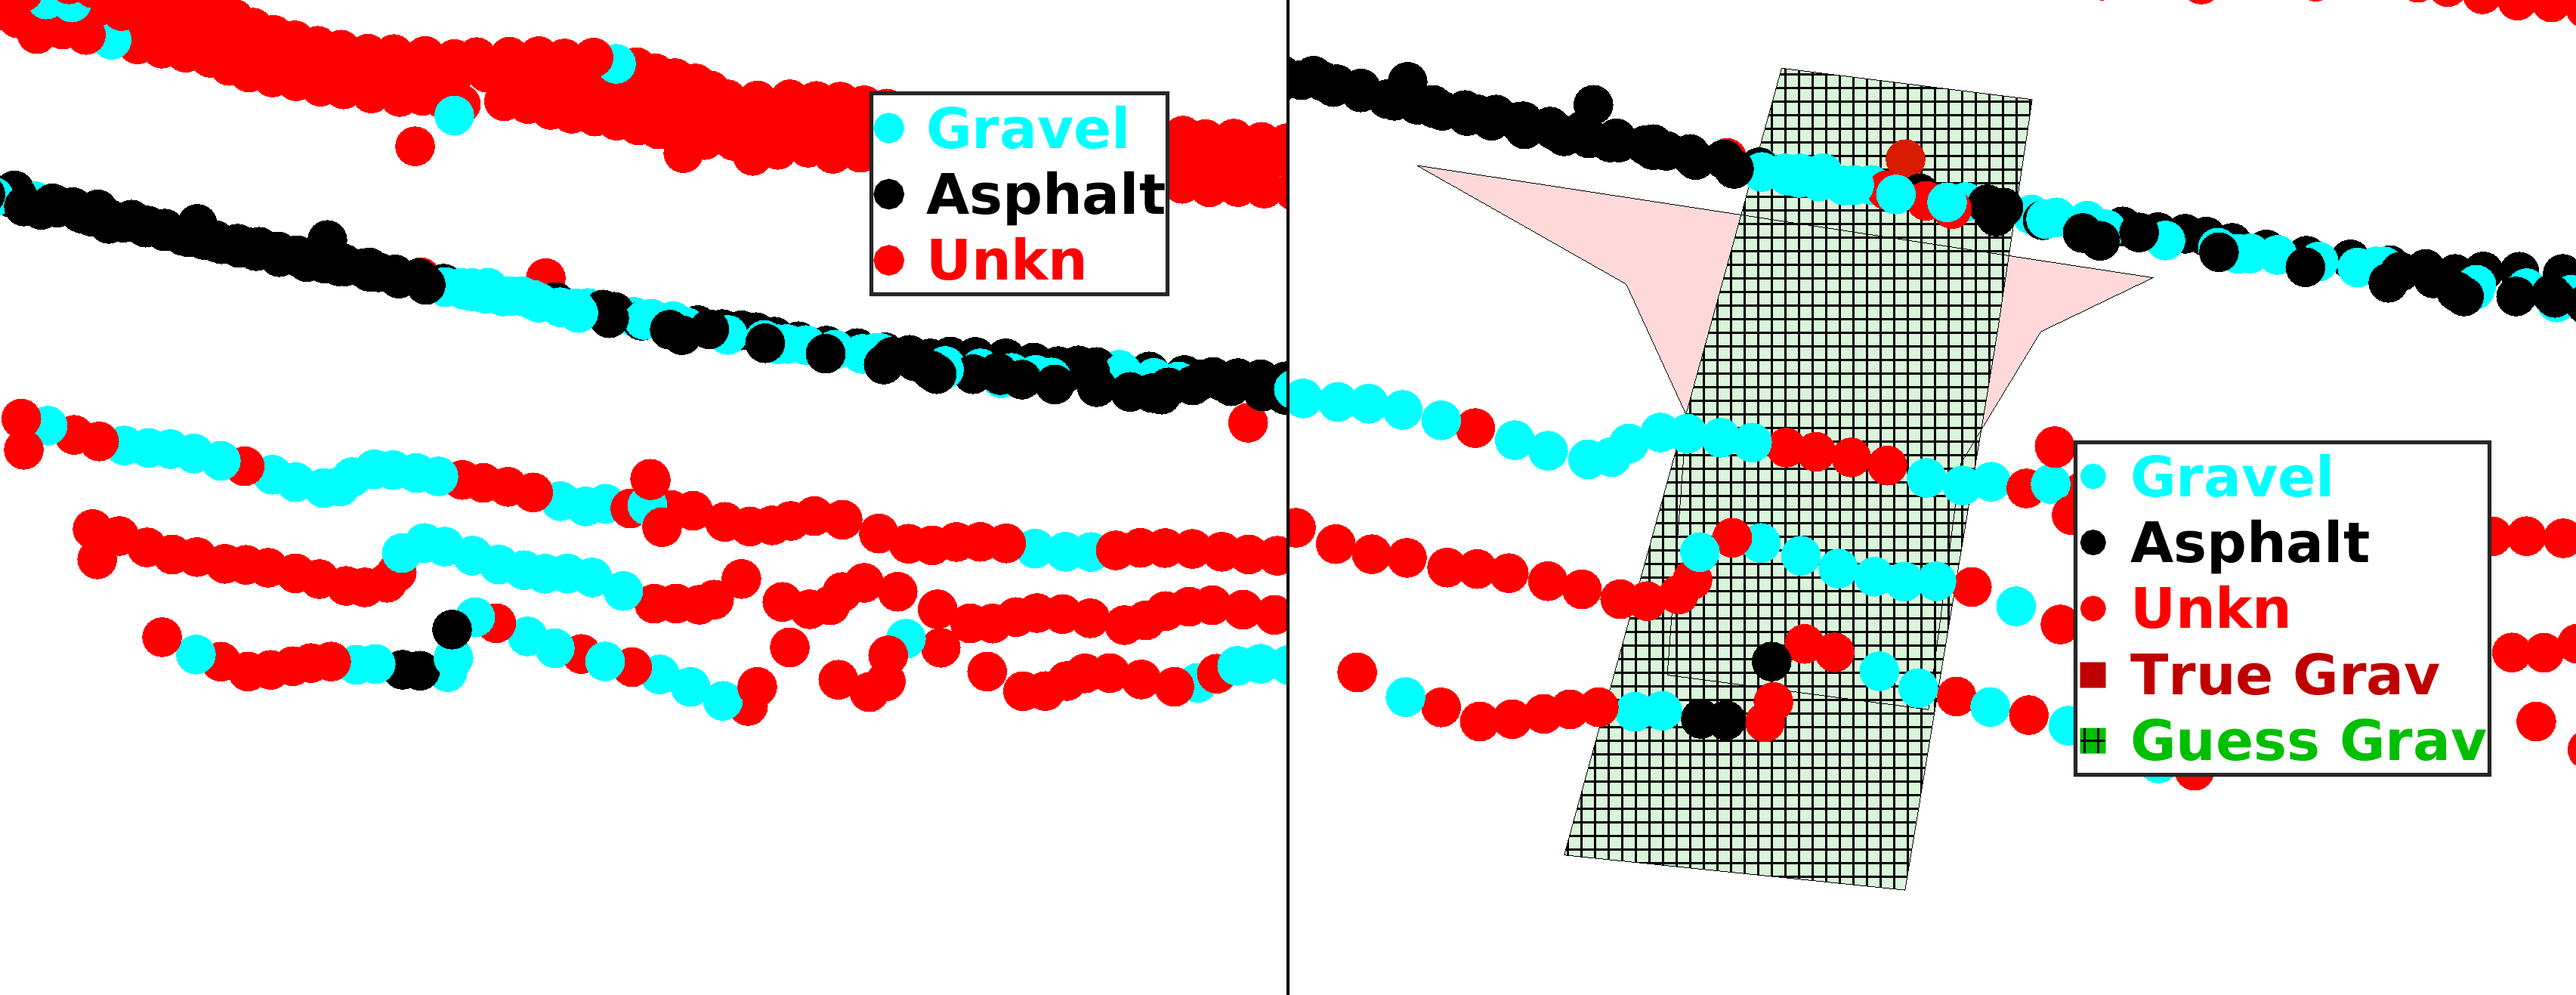
\includegraphics[width=0.9\linewidth]{figures/cross_channel_trend}
				\caption[Projected Guess vs Truth]{Gravel and asphalt surfaces were manually guessed based on trends between channels and compared to actual road-surface areas.}
				\label{fig:rm_db_4_toc}
			\end{figure}
				
	\section{Results}
	
		{Five drive-bys of Blackburn Road, which has three intersecting gravel parking lots and driveways, were completed, and scanning LiDAR, GPS, and IMU data was collected. Training data was generated using MATLAB to extract LiDAR data from rosbags, and RDF classification algorithms were generated. Testing consecutive scans was completed by post processing rosbags that contained scanning LiDAR, GPS, and IMU data. Physical distances between the GPS, IMU, and LiDAR were rectified by measuring the distance between the modules. Rotational reference frames between the GPS, IMU, and LiDAR were rectified by applying appropriate rotational matrices. Transformation matrices were created by considering the GPS position and the IMU's roll, pitch, and yaw data. Three scanning LiDAR arcs from three channels in front of the vehicle were classified. Translation and rotation was applied to the averaged x, y, and z coordinates of each arc's terrain classification results. Consecutive scanning LiDAR data was projected on manually classified truth areas representing road road surfaces (Figure \ref{fig:prepostadjust}) and percentages of terrain types per area were calculated.}
		
		\begin{table}[t]
			
			\centering{%
				\begin{tabular}{lrl}
					\toprule
					Gravel Areas \% 						& 74.97 	& \% Gravel \\
					Asphalt Area \%							& 87.05   	& \% Asphalt \\
					Side-of-Road \% 						& 77.47 	& \% Unknown\\
					Asphalt Road Detection 					& 100.00 	& \% True Pos. Detection Rate \\
					Gravel Driveway Detection 				& 93.33 	& \% True Pos. Detection Rate \\
					Misidentified Gravel Road Detection 	& 0.60 		&  Avg. False Pos. Detection Rate per Run\\
					\bottomrule
				\end{tabular}
			}
			\caption[Table]{Average Results\label{tab:1}}
		\end{table}
	
		{Classification of real-world data outside of the training data set presents difficulties to the generated Random Decision Forest Classifiers generated in this work. Due to the side of the road being re-grassed near a portion of the asphalt road, the terrain classification algorithm struggled to differentiate the dirt from gravel, leading to some misclassification of the side-of-road areas. Examination of the feature distribution shows a high amount of overlap (Fig. \ref{fig:dirt_v_gravel}). Exploitation of confidence scores to adjust results by requiring a very high confidence for positive gravel surface classification was explored. All gravel surfaces that did not meet a 80\% confidence score was re-labeled as \textit{unknown}, however these adjustment had either a negligible or detrimental impact on the final results. Higher confidence score requirements resulted in \textit{unknown} over-classification, while too low resulted in \textit{gravel} over-classification. Overall it was found that an average true-positive accuracy of all intercepting gravel surfaces was 74.97\% (Fig. \ref{fig:prepostadjust}). If any asphalt miss-classification on the gravel areas is included, the average true-positive road detection accuracy increases to 79.18\%. It was found that an average true-positive accuracy of all asphalt surfaces was 87.05\%. Due to recent construction, discovered asphalt accuracy was artificially lowered due to the area in front of a gravel driveway being contaminated with gravel. It was found that an average of 18.55\% of asphalt areas were classified as gravel because of contamination. Differentiation between gravel road surfaces and surrounding terrain is necessary to determine boundaries for trajectory tracking and navigation. Overall average distribution for \textit{unknown} terrain class within side-of-road areas was found to be 77.94\%, which is lower than expected due to the side of the road being re-grassed. It is acknowledged by the authors that the classification algorithm must yield a result that most closely matches one of the trained classes, which led to lower accuracy scores in these circumstances. It is difficult to determine if these results are comparable to similar research, as found research classifies larger data sets. For example, work completed by Laible et. al. \cite{levi_3d_2012_light} used $\sim1200$ data points, compared to the $\sim28$ data points per arc in this work. Overall discovered accuracy levels may be sufficient for the purpose of identifying asphalt and gravel roads by considering trends between classified arcs.}
		
		\begin{figure}[H]
			\centering
			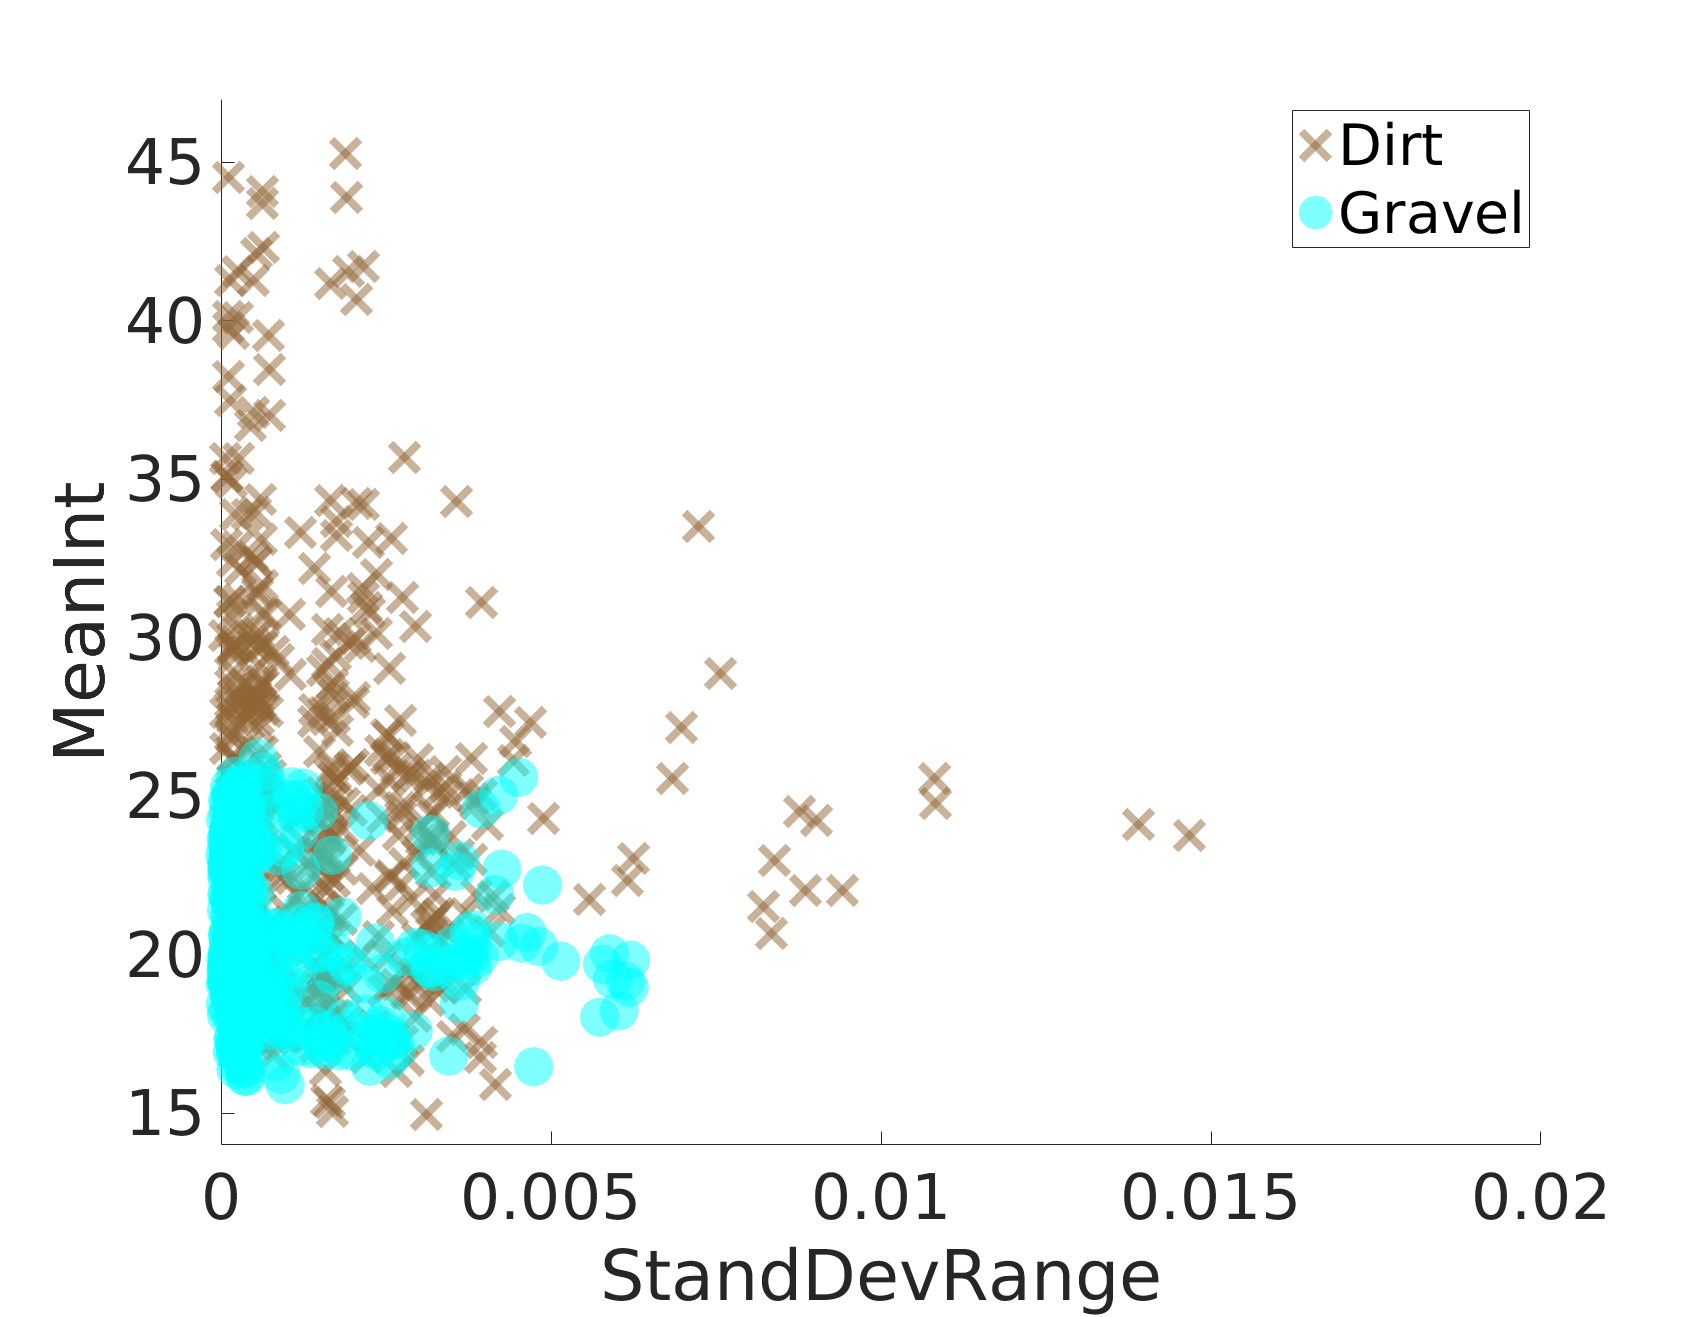
\includegraphics[width=0.75\linewidth]{figures/dirt_v_gravel2}
			\caption[Re-grassed Dirt vs Gravel]{Side-of-road detection accuracy was diminished due to overlapping features between dirt and gravel. }
			\label{fig:dirt_v_gravel}
		\end{figure}
	
		\begin{figure}[H]
			\centering
			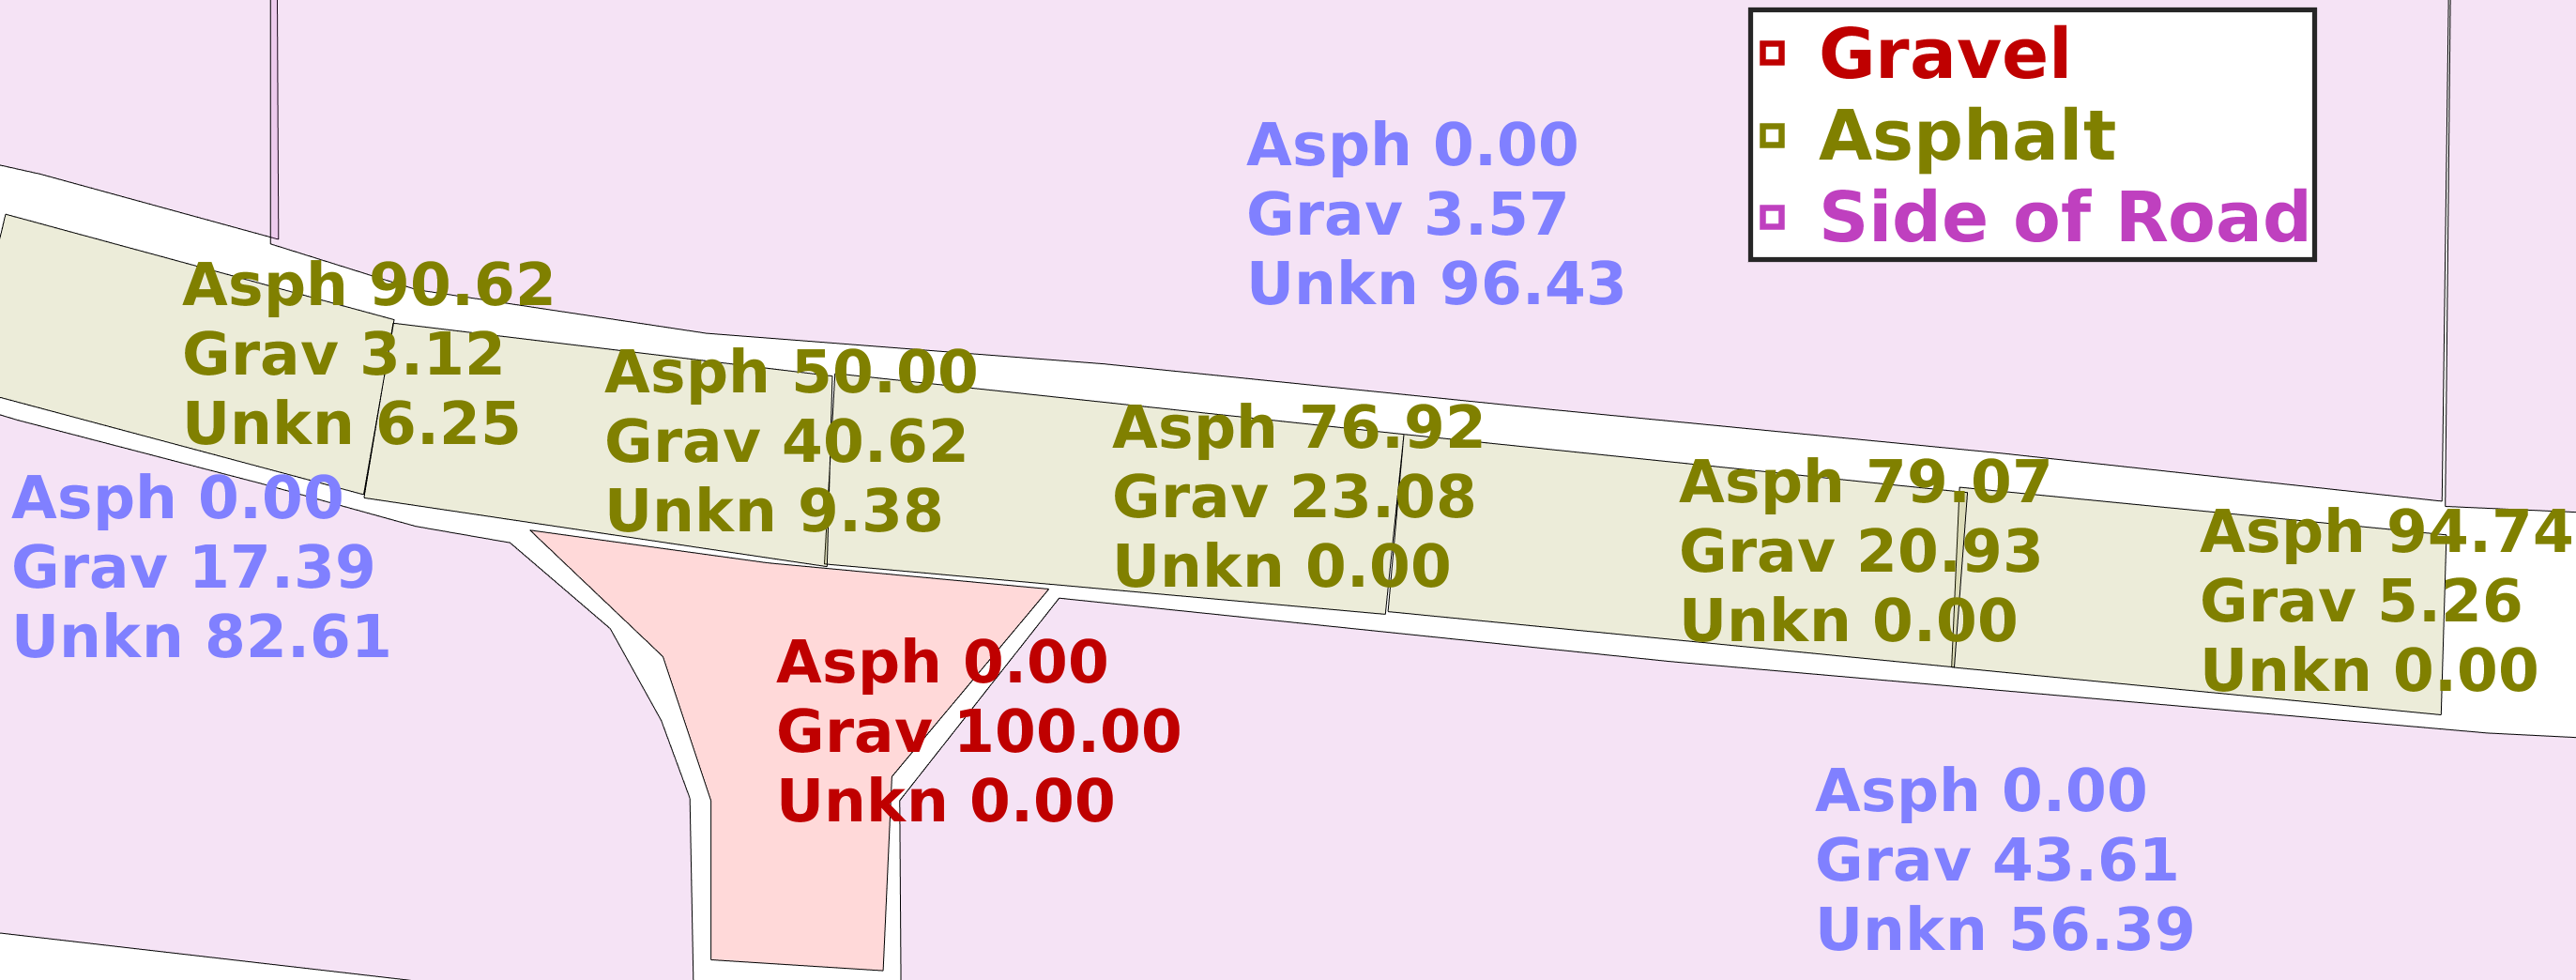
\includegraphics[width=0.75\linewidth]{figures/range_actual_rm_db_4_area_score}
			\caption[Area Scores]{Per-area scores were calculated, indicating algorithm unmarked road detection accuracy. Note that the asphalt area in front of the gravel driveway has significant \textit{gravel} classification due to construction. These results are included with the overall asphalt classification score}
			\label{fig:prepostadjust}
		\end{figure}
	
		{Classified point clouds were manually examined for 'best guess' locations for gravel and asphalt surfaces. Two out of three positive gravel identifications must be made on each channel, be evenly spaced, and be relatively co-planar to other road surface guesses in order for a positive guess for an asphalt or gravel surface to be made (Fig. \ref{fig:rm_db_4_toc}). Driveways $1$ and $2$ were detected in all five drive-bys, driveway $3$ was detected in four leading to an 91.67\% accuracy in intercepting gravel road detection. It was found that in three drive-bys there was a false positive driveway detection, however the location of the false-positives were not repeated in any of the other drivebys. In all drive-bys the asphalt road was accurately detected. }
	
		{Classification was completed using Ubuntu 18.04 and an AMD Ryzen 9 5900X 12 core 24 thread. Rate of classification for all nine areas of interest in a single scan was found to be an average of 35.19 ms using a single core (Fig. \ref{fig:per_arc_classification_time}) or 316.68 ms per 360 degree scan. When utilizing all 24 cores during classification a rate of 13.19 ms per 360 scan. Extrapolating from the distance traveled during a drive-by, a hypothetical 71.39 feet per second or 48.68 miles per hour may be possible. Further optimization may increase this speed, however implementing real-time classification was not a focus of this work.}
		
		\begin{figure}[H]
			\centering
			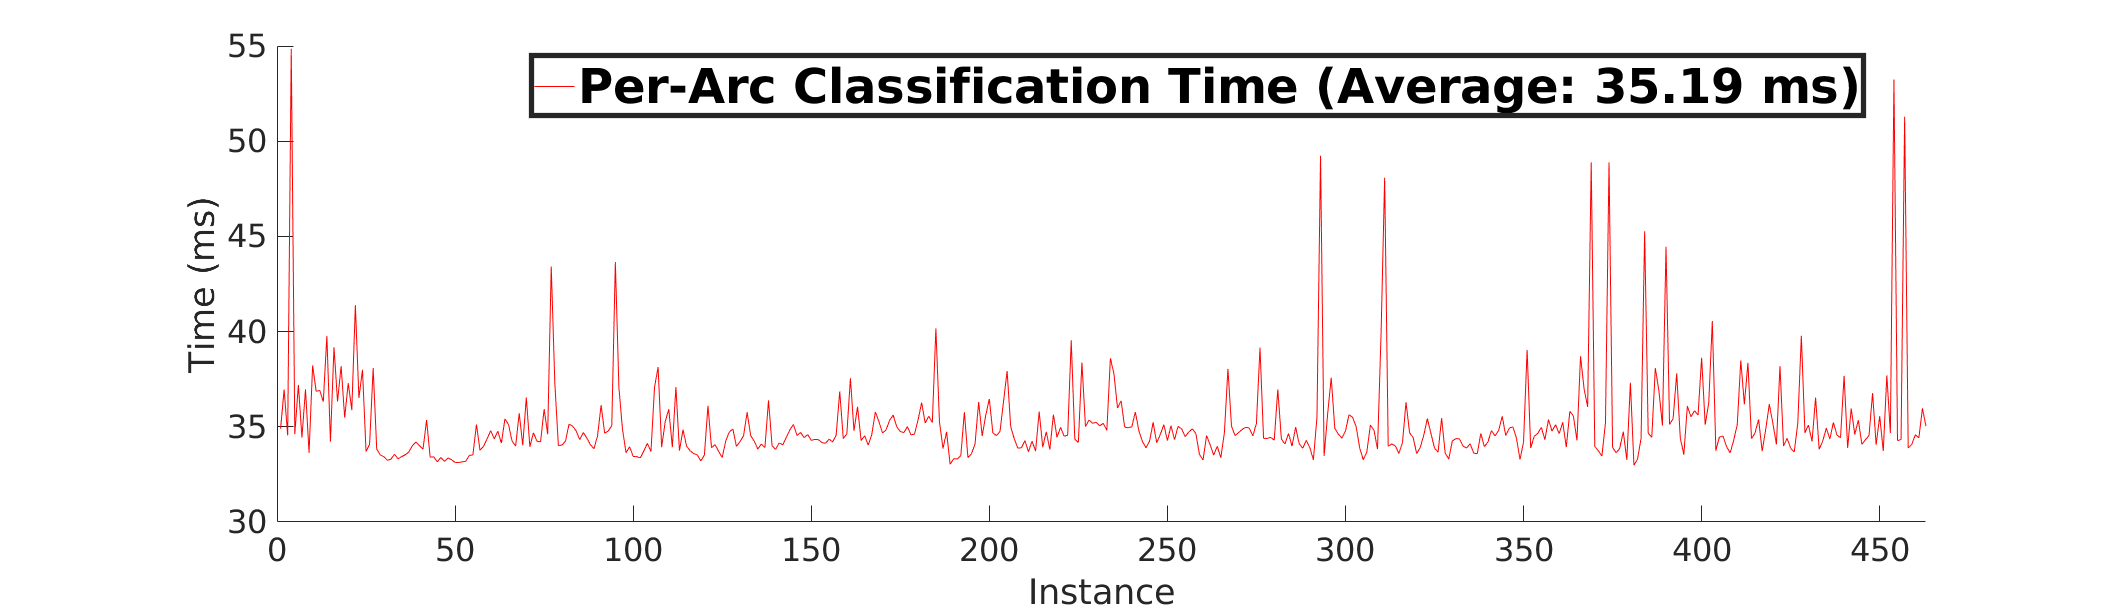
\includegraphics[width=0.75\linewidth]{figures/per_arc_classification_time}
			\caption[Per-Arc Time]{Per-arc classification time}
			\label{fig:per_arc_classification_time}
		\end{figure}

% 		(Fig. \ref{fig:per_scan_classification_rate})		
%		\begin{figure}[H]
%			\centering
%			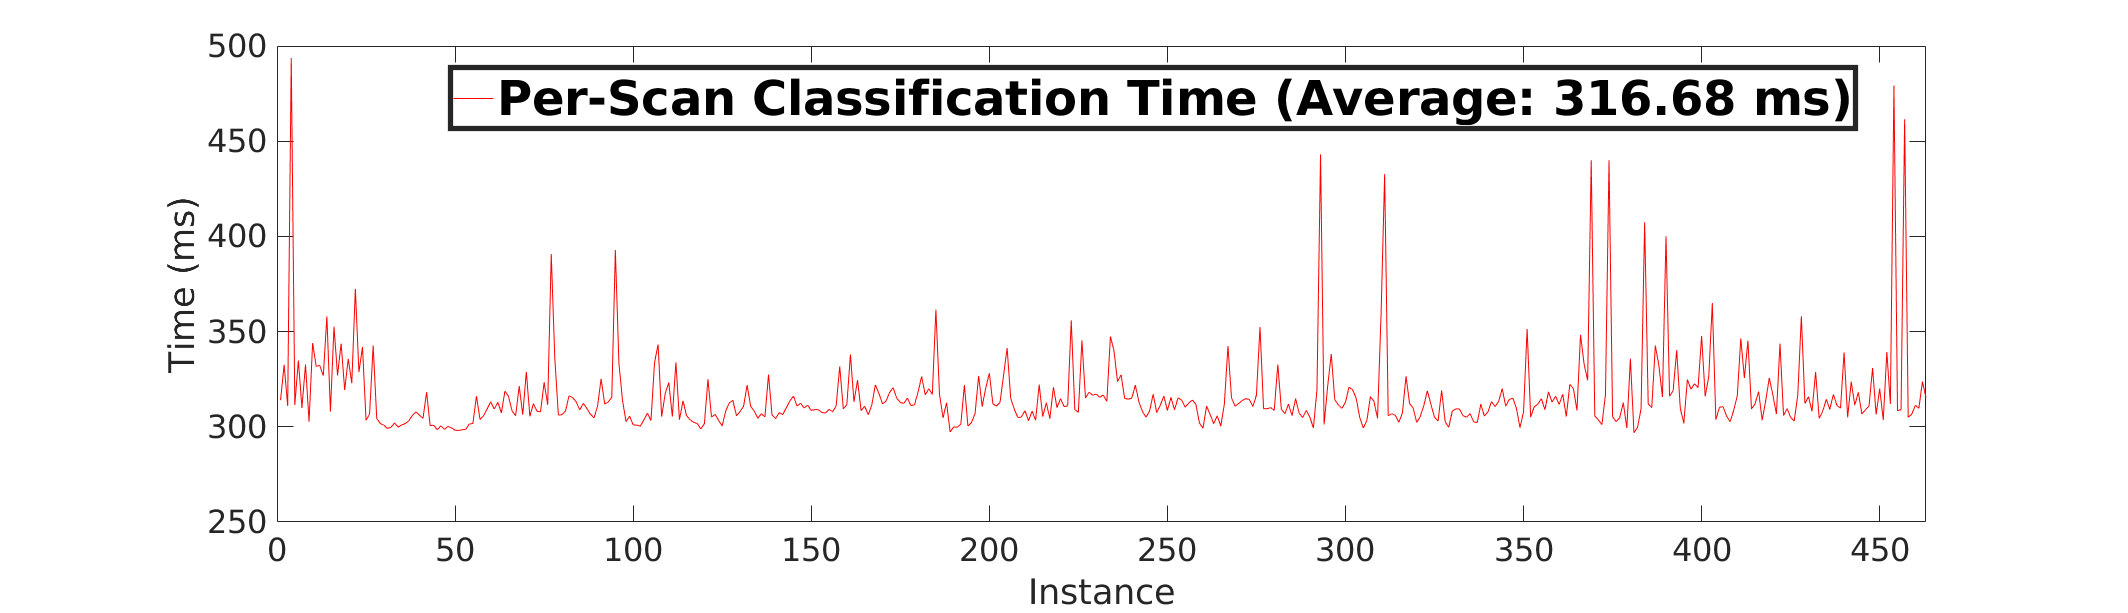
\includegraphics[width=0.75\linewidth]{figures/per_scan_classification_rate}
%			\caption[Per-Scan Time]{Per-scan classification time}
%			\label{fig:per_scan_classification_rate}
%		\end{figure}

	
	%%%%% Conclusions %%%%%%%%%%%%%%%%%%%%%%%%%%%%%%%
	
	\section{Conclusion}
	
		% Summary of Work & Closing Statements
		{High definition scanning LiDAR and GPS data was gathered on Blackburn Road and intersecting gravel lots in Athens Ohio. Properties describing surface roughness and remission data were extracted and used to train Random Decision Forests. Terrain classification of consecutive scans compared to manually detected road surface areas yielded accuracy scores for gauging algorithm capability for gravel surface detection. It was found that a true-positive accuracy for gravel and asphalt surfaces was 67.54\% and 87.05\% respectively at an estimated rate of 13.19 milliseconds per 360 degree scan. Classified point clouds were examined and gravel areas were projected and compared with actual gravel surface areas. Overlapping results between detected and actual road surface areas resulted in 91.67\% intersecting gravel road detection accuracy. In conjunction with the overlapping areas and the high true-positive detection accuracy of gravel surfaces, this method of gravel road detection is promising for future exploration of additional roads and road surfaces. Work as described addressed the problem of road surface detection on unmarked gravel and chipseal roads. The described work was a method of detecting physical unmarked gravel and chipseal roads by using a terrain classification approach to predicting road surface area. The impact of this work is that autonomous vehicles using the developed method may be able to detect unmarked gravel and chipseal road surfaces, allowing autonomous operations on 1.5 million miles of previously undetected rural roads.} 
	
% For peer review papers, you can put extra information on the cover
% page as needed:
% \ifCLASSOPTIONpeerreview
% \begin{center} \bfseries EDICS Category: 3-BBND \end{center}
% \fi
%
% For peerreview papers, this IEEEtran command inserts a page break and
% creates the second title. It will be ignored for other modes.
\IEEEpeerreviewmaketitle




% if have a single appendix:
%\appendix[Proof of the Zonklar Equations]
% or
%\appendix  % for no appendix heading
% do not use \section anymore after \appendix, only \section*
% is possibly needed

% use appendices with more than one appendix
% then use \section to start each appendix
% you must declare a \section before using any
% \subsection or using \label (\appendices by itself
% starts a section numbered zero.)
%


\appendices
%\section{Equations}

%\begin{equation}\label{eqn:MLS}
%	\left[ {\begin{array}{cc}
%			\sum_{i=1}^{m} x_i z_i \\
%			\sum_{i=1}^{m} y_i z_i \\
%			\sum_{i=1}^{m} z_i \\
%			
%	\end{array} } \right]
%	=
%	\left[ {\begin{array}{ccc}
%			\sum_{i=1}^{m} x_i^2 		& \sum_{i=1}^{m} x_i y_i 		& \sum_{i=1}^{m} x_i \\
%			\sum_{i=1}^{m} x_i y_i 		& \sum_{i=1}^{m} y_i^2 			& \sum_{i=1}^{m} y_i \\
%			\sum_{i=1}^{m} x_i 			& \sum_{i=1}^{m} y_i 			& \sum_{i=1}^{m} 1   \\
%	\end{array} } \right]
%	\left[ {\begin{array}{cc}
%			A\\
%			B\\
%			C\\
%	\end{array} } \right]
%\end{equation}
%\centering
%{Method of Least Squares Planar Projection}


% you can choose not to have a title for an appendix
%% if you want by leaving the argument blank
%\section{}
%Appendix two text goes here.


% use section* for acknowledgment
\justifying
\section*{Acknowledgment}


	{The authors would like to acknowledge the Ohio Department of Transportation, United States Department of Transportation, and the Drive Ohio Automated Driving Systems Project for making this work possible.}


% Can use something like this to put references on a page
% by themselves when using endfloat and the captionsoff option.
\ifCLASSOPTIONcaptionsoff
\newpage
\fi



% trigger a \newpage just before the given reference
% number - used to balance the columns on the last page
% adjust value as needed - may need to be readjusted if
% the document is modified later
%\IEEEtriggeratref{8}
% The "triggered" command can be changed if desired:
%\IEEEtriggercmd{\enlargethispage{-5in}}

% references section

% can use a bibliography generated by BibTeX as a .bbl file
% BibTeX documentation can be easily obtained at:
% http://mirror.ctan.org/biblio/bibtex/contrib/doc/
% The IEEEtran BibTeX style support page is at:
% http://www.michaelshell.org/tex/ieeetran/bibtex/
%\bibliographystyle{IEEEtran}
% argument is your BibTeX string definitions and bibliography database(s)
%\bibliography{IEEEabrv,../bib/paper}
%
% <OR> manually copy in the resultant .bbl file
% set second argument of \begin to the number of references
% (used to reserve space for the reference number labels box)


	\bibliographystyle{ieeetr}  
	\bibliography{resources.bib} 





% that's all folks
\end{document}